% Options for packages loaded elsewhere
\PassOptionsToPackage{unicode}{hyperref}
\PassOptionsToPackage{hyphens}{url}
%
\documentclass[
]{article}
\usepackage{amsmath,amssymb}
\usepackage{lmodern}
\usepackage{ifxetex,ifluatex}
\ifnum 0\ifxetex 1\fi\ifluatex 1\fi=0 % if pdftex
  \usepackage[T1]{fontenc}
  \usepackage[utf8]{inputenc}
  \usepackage{textcomp} % provide euro and other symbols
\else % if luatex or xetex
  \usepackage{unicode-math}
  \defaultfontfeatures{Scale=MatchLowercase}
  \defaultfontfeatures[\rmfamily]{Ligatures=TeX,Scale=1}
\fi
% Use upquote if available, for straight quotes in verbatim environments
\IfFileExists{upquote.sty}{\usepackage{upquote}}{}
\IfFileExists{microtype.sty}{% use microtype if available
  \usepackage[]{microtype}
  \UseMicrotypeSet[protrusion]{basicmath} % disable protrusion for tt fonts
}{}
\makeatletter
\@ifundefined{KOMAClassName}{% if non-KOMA class
  \IfFileExists{parskip.sty}{%
    \usepackage{parskip}
  }{% else
    \setlength{\parindent}{0pt}
    \setlength{\parskip}{6pt plus 2pt minus 1pt}}
}{% if KOMA class
  \KOMAoptions{parskip=half}}
\makeatother
\usepackage{xcolor}
\IfFileExists{xurl.sty}{\usepackage{xurl}}{} % add URL line breaks if available
\IfFileExists{bookmark.sty}{\usepackage{bookmark}}{\usepackage{hyperref}}
\hypersetup{
  pdftitle={IB-202P Posthoc Analyses},
  pdfauthor={Fred Hutch Team},
  hidelinks,
  pdfcreator={LaTeX via pandoc}}
\urlstyle{same} % disable monospaced font for URLs
\usepackage[margin=1in]{geometry}
\usepackage{graphicx}
\makeatletter
\def\maxwidth{\ifdim\Gin@nat@width>\linewidth\linewidth\else\Gin@nat@width\fi}
\def\maxheight{\ifdim\Gin@nat@height>\textheight\textheight\else\Gin@nat@height\fi}
\makeatother
% Scale images if necessary, so that they will not overflow the page
% margins by default, and it is still possible to overwrite the defaults
% using explicit options in \includegraphics[width, height, ...]{}
\setkeys{Gin}{width=\maxwidth,height=\maxheight,keepaspectratio}
% Set default figure placement to htbp
\makeatletter
\def\fps@figure{htbp}
\makeatother
\setlength{\emergencystretch}{3em} % prevent overfull lines
\providecommand{\tightlist}{%
  \setlength{\itemsep}{0pt}\setlength{\parskip}{0pt}}
\setcounter{secnumdepth}{5}
\usepackage{booktabs}
\usepackage{longtable}
\usepackage{array}
\usepackage{multirow}
\usepackage{wrapfig}
\usepackage{float}
\usepackage{colortbl}
\usepackage{pdflscape}
\usepackage{tabu}
\usepackage{threeparttable}
\usepackage{threeparttablex}
\usepackage[normalem]{ulem}
\usepackage{makecell}
\usepackage{xcolor}
\ifluatex
  \usepackage{selnolig}  % disable illegal ligatures
\fi

\title{IB-202P Posthoc Analyses}
\author{Fred Hutch Team}
\date{}

\begin{document}
\maketitle

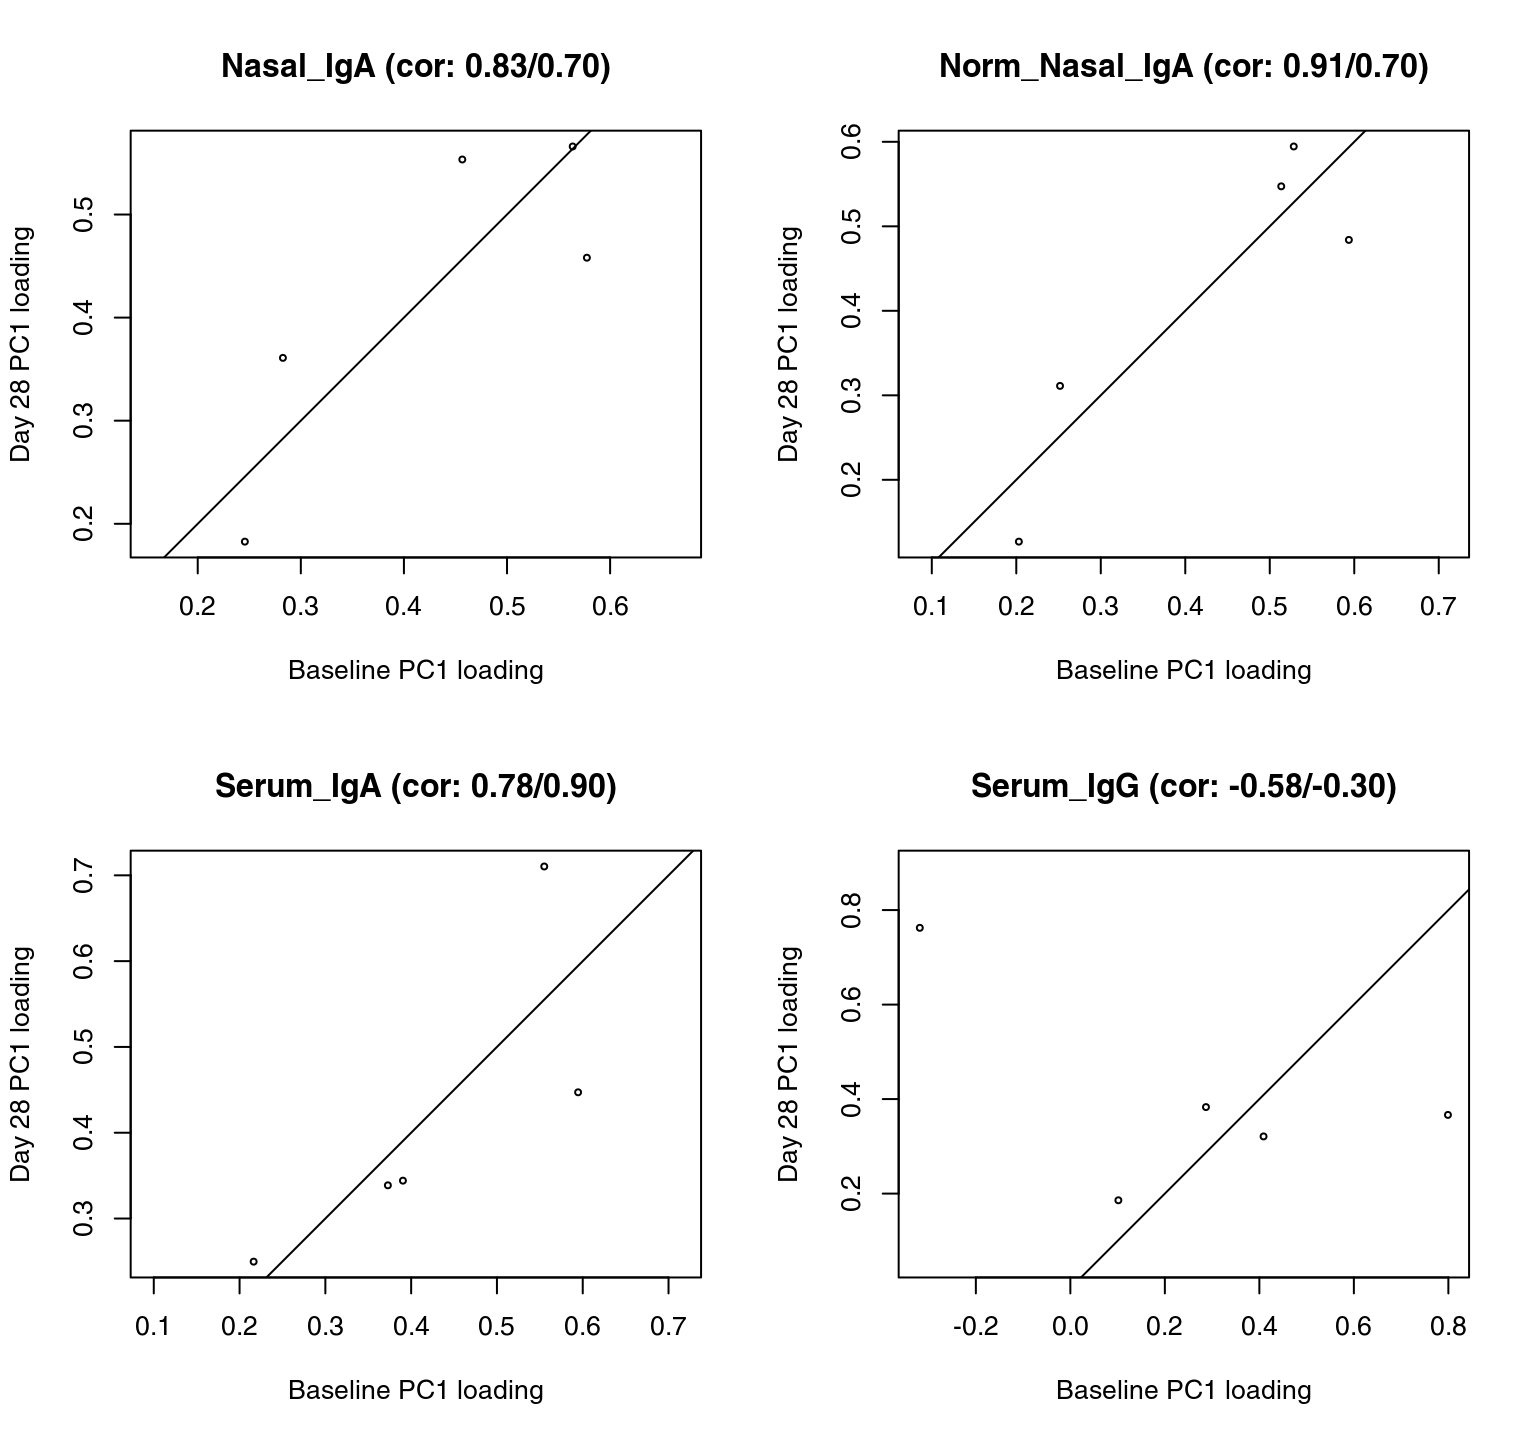
\includegraphics{posthoc_analyses_files/figure-latex/pc1-1.pdf}

\begin{verbatim}
## 
## Barnard's Unconditional Test
## 
##            Treatment I Treatment II
## Outcome I            4           12
## Outcome II          12            8
## 
## Null hypothesis: Treatments have no effect on the outcomes
## Score statistic = 2.1
## Nuisance parameter = 0.813 (One sided), 0.618 (Two sided)
## P-value = 0.0218294 (One sided), 0.0402774 (Two sided)
\end{verbatim}

\begin{verbatim}
## 
## Barnard's Unconditional Test
## 
##            Treatment I Treatment II
## Outcome I            4           14
## Outcome II          12            6
## 
## Null hypothesis: Treatments have no effect on the outcomes
## Score statistic = 2.68328
## Nuisance parameter = 0.815 (One sided), 0.5 (Two sided)
## P-value = 0.00416738 (One sided), 0.00787482 (Two sided)
\end{verbatim}

\begin{verbatim}
## 
## Barnard's Unconditional Test
## 
##            Treatment I Treatment II
## Outcome I            7           14
## Outcome II          14           10
## 
## Null hypothesis: Treatments have no effect on the outcomes
## Score statistic = 1.67705
## Nuisance parameter = 0.431 (One sided), 0.431 (Two sided)
## P-value = 0.0516969 (One sided), 0.0928395 (Two sided)
\end{verbatim}

\begin{verbatim}
## 
## Barnard's Unconditional Test
## 
##            Treatment I Treatment II
## Outcome I            7           16
## Outcome II          14            7
## 
## Null hypothesis: Treatments have no effect on the outcomes
## Score statistic = 2.40335
## Nuisance parameter = 0.522 (One sided), 0.539 (Two sided)
## P-value = 0.010194 (One sided), 0.0188403 (Two sided)
\end{verbatim}

\begin{tabular}{l|c|c}
\hline
  & Sex & Age\\
\hline
 & 1.27 (CI=0.48,3.37, p=0.633) & 0.97 (CI=0.91,1.03, p=0.324)\\
\hline
\end{tabular}

\begin{verbatim}
## Warning in wilcox.test.default(x = c(25L, 43L, 24L, 45L, 39L, 21L, 35L, : cannot
## compute exact p-value with ties
\end{verbatim}

\begin{verbatim}
## Warning in wilcox.test.default(x = c(29L, 23L, 36L, 21L, 19L, 23L, 36L), :
## cannot compute exact p-value with ties
\end{verbatim}

\begin{verbatim}
## Warning in wilcox.test.default(x = c(24L, 45L, 39L, 21L, 35L, 22L, 35L, : cannot
## compute exact p-value with ties
\end{verbatim}

\begin{verbatim}
## Warning in wilcox.test.default(x = c(21L, 19L, 23L, 36L), y = c(49L, 28L, :
## cannot compute exact p-value with ties
\end{verbatim}

\begin{tabular}{l|l|l|l|l}
\hline
  & PP, Wilcox & PPAI, Wilcox & PP, t & PPAI, t\\
\hline
BPZE1 & 0.331 & 0.437 & 0.342 & 0.369\\
\hline
PBO & 0.092 & 0.113 & 0.055 & 0.072\\
\hline
\end{tabular}

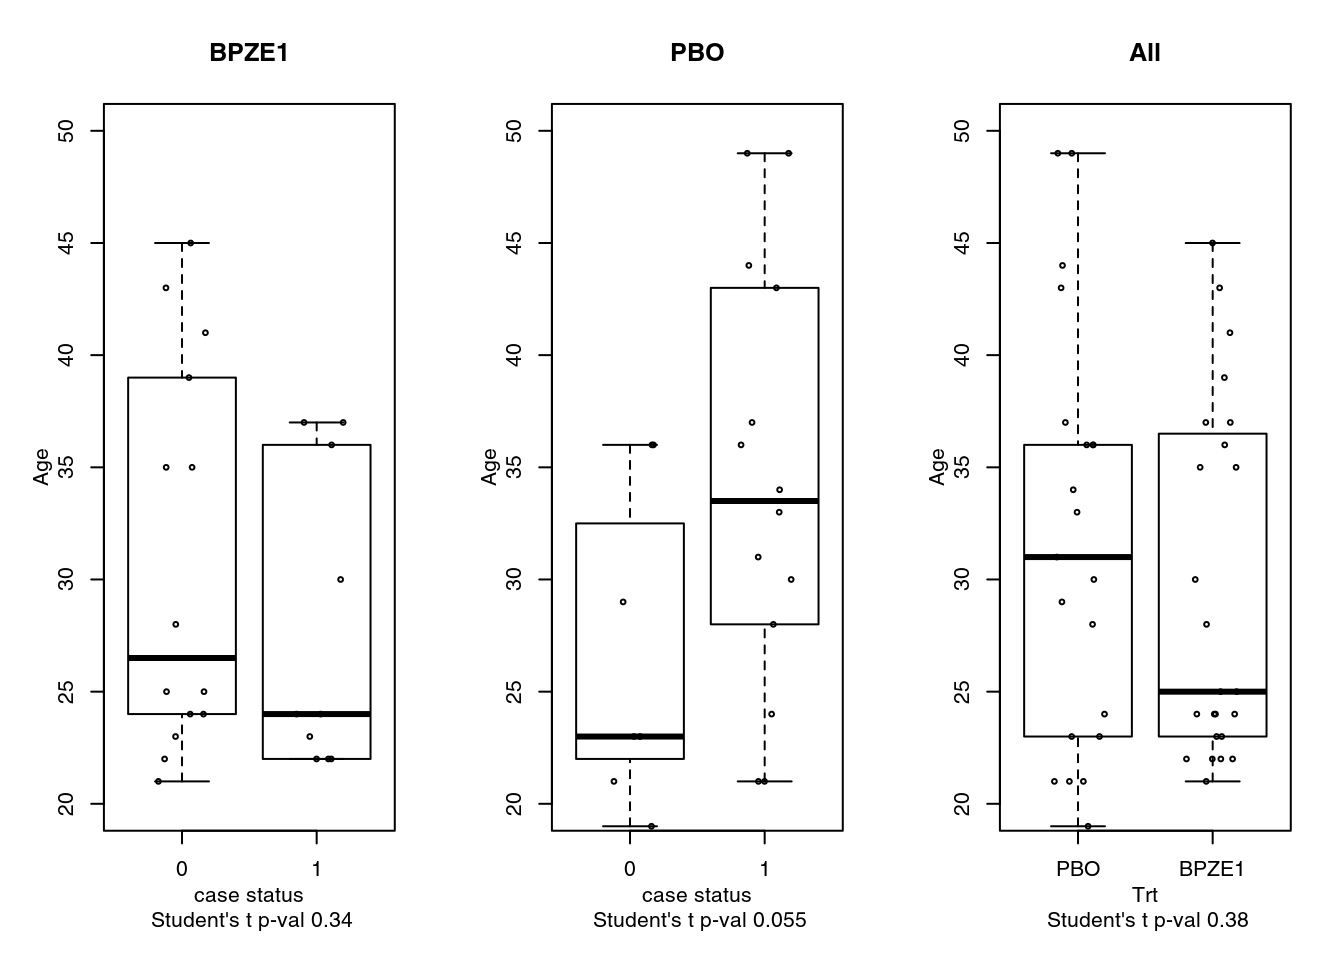
\includegraphics{posthoc_analyses_files/figure-latex/covariates selection with two sample comparison-1.pdf}

\begin{verbatim}
## [1] 0.69683
\end{verbatim}

\begin{verbatim}
## [1] 0.6594427
\end{verbatim}

\begin{verbatim}
## [1] 0.7683107
\end{verbatim}

\begin{verbatim}
##             1                                 
## (Intercept) "1.24 (CI= 0.79,1.69, p=<0.001)**"
## Age         "0.01 (CI=-0.01,0.02, p=0.395)"
\end{verbatim}

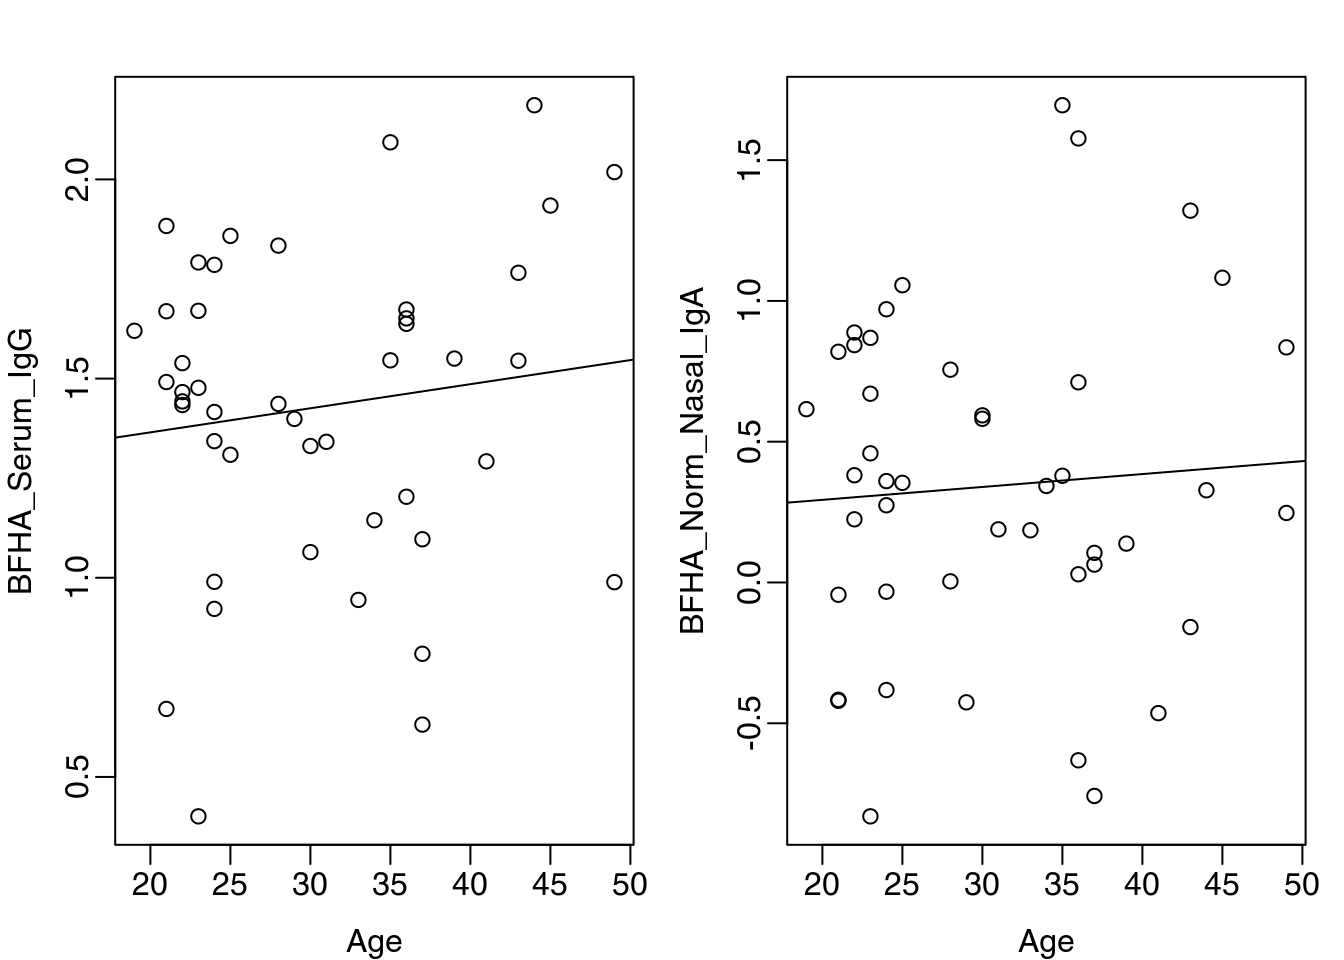
\includegraphics{posthoc_analyses_files/figure-latex/covariates selection with two sample comparison-2.pdf}

\begin{verbatim}
##             1                              
## (Intercept) "0.20 (CI=-0.47,0.87, p=0.547)"
## Age         "0.00 (CI=-0.02,0.03, p=0.665)"
\end{verbatim}

\begin{tabular}{>{}l|>{}c|>{}c|>{}c|c}
\hline
\multicolumn{1}{c|}{Wilcox} & \multicolumn{2}{c|}{PP} & \multicolumn{2}{c}{PPAI} \\
\cline{1-1} \cline{2-3} \cline{4-5}
  & BPZE1 & PBO & BPZE1 & PBO\\
\hline
Day28 & 0.192 & 0.031 & 0.208 & 0.030\\
\hline
B & 0.154 & 0.025 & 0.473 & 0.020\\
\hline
D28/B & 0.371 & 0.585 & 0.792 & 0.521\\
\hline
\end{tabular}

\begin{tabular}{>{}l|>{}c|>{}c|>{}c|c}
\hline
\multicolumn{1}{c|}{t test} & \multicolumn{2}{c|}{PP} & \multicolumn{2}{c}{PPAI} \\
\cline{1-1} \cline{2-3} \cline{4-5}
  & BPZE1 & PBO & BPZE1 & PBO\\
\hline
Day28 & 0.106 & 0.044 & 0.099 & 0.019\\
\hline
B & 0.078 & 0.033 & 0.315 & 0.029\\
\hline
D28/B & 0.808 & 0.159 & 0.641 & 0.236\\
\hline
\end{tabular}

\begin{tabular}{>{}l|>{}c|>{}c|>{}c|c}
\hline
\multicolumn{1}{c|}{Poisson MBN} & \multicolumn{2}{c|}{PP} & \multicolumn{2}{c}{PPAI} \\
\cline{1-1} \cline{2-3} \cline{4-5}
  & BPZE1 & PBO & BPZE1 & PBO\\
\hline
Day28 & 0.039 & 0.067 & 0.044 & 0.082\\
\hline
B & 0.039 & 0.035 & 0.343 & 0.048\\
\hline
D28/B & 0.818 & 0.162 & 0.648 & 0.352\\
\hline
\end{tabular}

\begin{tabular}{>{}l|>{}c|>{}c|>{}c|c}
\hline
\multicolumn{1}{c|}{Poisson MD} & \multicolumn{2}{c|}{PP} & \multicolumn{2}{c}{PPAI} \\
\cline{1-1} \cline{2-3} \cline{4-5}
  & BPZE1 & PBO & BPZE1 & PBO\\
\hline
Day28 & 0.031 & 0.060 & 0.033 & 0.062\\
\hline
B & 0.037 & 0.027 & 0.400 & 0.036\\
\hline
D28/B & 0.861 & 0.077 & 0.691 & 0.199\\
\hline
\end{tabular}

\begin{tabular}{>{}l|>{}c|>{}c|>{}c|c}
\hline
\multicolumn{1}{c|}{Poisson} & \multicolumn{2}{c|}{PP} & \multicolumn{2}{c}{PPAI} \\
\cline{1-1} \cline{2-3} \cline{4-5}
  & BPZE1 & PBO & BPZE1 & PBO\\
\hline
Day28 & 0.018 & 0.036 & 0.018 & 0.029\\
\hline
B & 0.019 & 0.014 & 0.292 & 0.012\\
\hline
D28/B & 0.803 & 0.056 & 0.609 & 0.134\\
\hline
\end{tabular}

\begin{verbatim}
## Error in if (bold) {: missing value where TRUE/FALSE needed
\end{verbatim}

\begin{verbatim}
## Error in if (bold) {: missing value where TRUE/FALSE needed
\end{verbatim}

\begin{verbatim}
## Error in if (bold) {: missing value where TRUE/FALSE needed
\end{verbatim}

\begin{verbatim}
## Error in if (bold) {: missing value where TRUE/FALSE needed
\end{verbatim}

\begin{verbatim}
## Error in if (bold) {: missing value where TRUE/FALSE needed
\end{verbatim}

\begin{verbatim}
## Error in if (bold) {: missing value where TRUE/FALSE needed
\end{verbatim}

\begin{tabular}{>{}l|>{}c|>{}c|>{}c|>{}c|c}
\hline
\multicolumn{1}{c|}{PPAI prim} & \multicolumn{1}{c|}{WCE} & \multicolumn{1}{c|}{FHA} & \multicolumn{1}{c|}{FIM} & \multicolumn{1}{c|}{PRN} & \multicolumn{1}{c}{PT} \\
\cline{1-1} \cline{2-2} \cline{3-3} \cline{4-4} \cline{5-5} \cline{6-6}
Nasal\_IgA & 0.665 & 0.488 & 0.699 & 0.997 & 0.407\\
\hline
Norm\_sIgA & 0.082 & 0.044 & 0.224 & 0.425 & 0.742\\
\hline
Serum\_IgA & 0.058 & 0.477 & 0.119 & 0.325 & 0.274\\
\hline
Serum\_IgG & 0.446 & 0.002 & 0.646 & 0.109 & 0.032\\
\hline
\end{tabular}

\begin{tabular}{>{}l|>{}c|>{}c|>{}c|>{}c|c}
\hline
\multicolumn{1}{c|}{PPAI alt} & \multicolumn{1}{c|}{WCE} & \multicolumn{1}{c|}{FHA} & \multicolumn{1}{c|}{FIM} & \multicolumn{1}{c|}{PRN} & \multicolumn{1}{c}{PT} \\
\cline{1-1} \cline{2-2} \cline{3-3} \cline{4-4} \cline{5-5} \cline{6-6}
Nasal\_IgA & 0.392 & 0.385 & 0.191 & 0.574 & 0.865\\
\hline
Norm\_sIgA & 0.195 & 0.215 & 0.147 & 0.455 & 0.727\\
\hline
Serum\_IgA & 0.074 & 0.517 & 0.064 & 0.281 & 0.414\\
\hline
Serum\_IgG & 0.239 & 0.440 & 0.272 & 0.102 & 0.239\\
\hline
\end{tabular}

\begin{tabular}{>{}l|>{}c|>{}c|>{}c|>{}c|c}
\hline
\multicolumn{1}{c|}{PP prim} & \multicolumn{1}{c|}{WCE} & \multicolumn{1}{c|}{FHA} & \multicolumn{1}{c|}{FIM} & \multicolumn{1}{c|}{PRN} & \multicolumn{1}{c}{PT} \\
\cline{1-1} \cline{2-2} \cline{3-3} \cline{4-4} \cline{5-5} \cline{6-6}
Nasal\_IgA & 0.457 & 0.128 & 0.664 & 0.840 & 0.974\\
\hline
Norm\_sIgA & 0.191 & 0.039 & 0.368 & 0.875 & 0.499\\
\hline
Serum\_IgA & 0.526 & 0.411 & 0.756 & 0.886 & 0.663\\
\hline
Serum\_IgG & 0.773 & <0.001 & 0.321 & 0.470 & 0.145\\
\hline
\end{tabular}

\begin{tabular}{>{}l|>{}c|>{}c|>{}c|>{}c|c}
\hline
\multicolumn{1}{c|}{PP alt} & \multicolumn{1}{c|}{WCE} & \multicolumn{1}{c|}{FHA} & \multicolumn{1}{c|}{FIM} & \multicolumn{1}{c|}{PRN} & \multicolumn{1}{c}{PT} \\
\cline{1-1} \cline{2-2} \cline{3-3} \cline{4-4} \cline{5-5} \cline{6-6}
Nasal\_IgA & 0.214 & 0.110 & 0.186 & 0.406 & 0.470\\
\hline
Norm\_sIgA & 0.155 & 0.067 & 0.158 & 0.356 & 0.467\\
\hline
Serum\_IgA & 0.337 & 0.361 & 0.499 & 0.498 & 0.666\\
\hline
Serum\_IgG & 0.243 & 0.149 & 0.175 & 0.191 & 0.125\\
\hline
\end{tabular}

\begin{tabular}{>{}l|>{}c|>{}c|>{}c|>{}c|c}
\hline
\multicolumn{1}{c|}{PPAI prim} & \multicolumn{1}{c|}{WCE} & \multicolumn{1}{c|}{FHA} & \multicolumn{1}{c|}{FIM} & \multicolumn{1}{c|}{PRN} & \multicolumn{1}{c}{PT} \\
\cline{1-1} \cline{2-2} \cline{3-3} \cline{4-4} \cline{5-5} \cline{6-6}
Nasal\_IgA & 0.591 & 0.503 & 0.719 & 0.852 & 0.579\\
\hline
Norm\_sIgA & 0.099 & 0.074 & 0.271 & 0.587 & 0.632\\
\hline
Serum\_IgA & 0.100 & 0.704 & 0.126 & 0.524 & 0.262\\
\hline
Serum\_IgG & 0.452 & 0.007 & 0.782 & 0.206 & 0.065\\
\hline
\end{tabular}

\begin{tabular}{>{}l|>{}c|>{}c|>{}c|>{}c|c}
\hline
\multicolumn{1}{c|}{PPAI alt} & \multicolumn{1}{c|}{WCE} & \multicolumn{1}{c|}{FHA} & \multicolumn{1}{c|}{FIM} & \multicolumn{1}{c|}{PRN} & \multicolumn{1}{c}{PT} \\
\cline{1-1} \cline{2-2} \cline{3-3} \cline{4-4} \cline{5-5} \cline{6-6}
Nasal\_IgA & 0.333 & 0.408 & 0.130 & 0.736 & 0.643\\
\hline
Norm\_sIgA & 0.209 & 0.240 & 0.135 & 0.662 & 0.600\\
\hline
Serum\_IgA & 0.130 & 0.816 & 0.066 & 0.486 & 0.412\\
\hline
Serum\_IgG & 0.331 & 0.646 & 0.364 & 0.204 & 0.329\\
\hline
\end{tabular}

\begin{tabular}{>{}l|>{}c|>{}c|>{}c|>{}c|c}
\hline
\multicolumn{1}{c|}{PP prim} & \multicolumn{1}{c|}{WCE} & \multicolumn{1}{c|}{FHA} & \multicolumn{1}{c|}{FIM} & \multicolumn{1}{c|}{PRN} & \multicolumn{1}{c}{PT} \\
\cline{1-1} \cline{2-2} \cline{3-3} \cline{4-4} \cline{5-5} \cline{6-6}
Nasal\_IgA & 0.443 & 0.189 & 0.679 & 0.727 & 0.736\\
\hline
Norm\_sIgA & 0.259 & 0.111 & 0.484 & 0.899 & 0.407\\
\hline
Serum\_IgA & 0.803 & 0.672 & 0.849 & 0.586 & 0.609\\
\hline
Serum\_IgG & 0.794 & 0.002 & 0.424 & 0.659 & 0.189\\
\hline
\end{tabular}

\begin{tabular}{>{}l|>{}c|>{}c|>{}c|>{}c|c}
\hline
\multicolumn{1}{c|}{PP alt} & \multicolumn{1}{c|}{WCE} & \multicolumn{1}{c|}{FHA} & \multicolumn{1}{c|}{FIM} & \multicolumn{1}{c|}{PRN} & \multicolumn{1}{c}{PT} \\
\cline{1-1} \cline{2-2} \cline{3-3} \cline{4-4} \cline{5-5} \cline{6-6}
Nasal\_IgA & 0.200 & 0.181 & 0.097 & 0.494 & 0.294\\
\hline
Norm\_sIgA & 0.203 & 0.166 & 0.182 & 0.522 & 0.346\\
\hline
Serum\_IgA & 0.722 & 0.777 & 0.517 & 0.825 & 0.588\\
\hline
Serum\_IgG & 0.344 & 0.326 & 0.292 & 0.380 & 0.136\\
\hline
\end{tabular}

\begin{tabular}{>{}l|>{}c|>{}c|>{}c|>{}c|c}
\hline
\multicolumn{1}{c|}{PPAI prim} & \multicolumn{1}{c|}{WCE} & \multicolumn{1}{c|}{FHA} & \multicolumn{1}{c|}{FIM} & \multicolumn{1}{c|}{PRN} & \multicolumn{1}{c}{PT} \\
\cline{1-1} \cline{2-2} \cline{3-3} \cline{4-4} \cline{5-5} \cline{6-6}
Nasal\_IgA & 0.525 & 0.474 & 0.592 & 0.772 & 0.303\\
\hline
Norm\_sIgA & 0.884 & 0.343 & 0.384 & 0.964 & 0.358\\
\hline
Serum\_IgA & 0.770 & 0.630 & 0.854 & 0.795 & 0.662\\
\hline
Serum\_IgG & 0.357 & <0.001 & 0.155 & 0.607 & 0.368\\
\hline
\end{tabular}

\begin{tabular}{>{}l|>{}c|>{}c|>{}c|>{}c|c}
\hline
\multicolumn{1}{c|}{PPAI alt} & \multicolumn{1}{c|}{WCE} & \multicolumn{1}{c|}{FHA} & \multicolumn{1}{c|}{FIM} & \multicolumn{1}{c|}{PRN} & \multicolumn{1}{c}{PT} \\
\cline{1-1} \cline{2-2} \cline{3-3} \cline{4-4} \cline{5-5} \cline{6-6}
Nasal\_IgA & 0.896 & 0.479 & 0.314 & 0.726 & 0.422\\
\hline
Norm\_sIgA & 0.879 & 0.616 & 0.380 & 0.609 & 0.109\\
\hline
Serum\_IgA & 0.318 & 0.514 & 0.823 & 0.712 & 0.305\\
\hline
Serum\_IgG & 0.482 & 0.006 & 0.240 & 0.334 & 0.255\\
\hline
\end{tabular}

\begin{tabular}{>{}l|>{}c|>{}c|>{}c|>{}c|c}
\hline
\multicolumn{1}{c|}{PP prim} & \multicolumn{1}{c|}{WCE} & \multicolumn{1}{c|}{FHA} & \multicolumn{1}{c|}{FIM} & \multicolumn{1}{c|}{PRN} & \multicolumn{1}{c}{PT} \\
\cline{1-1} \cline{2-2} \cline{3-3} \cline{4-4} \cline{5-5} \cline{6-6}
Nasal\_IgA & 0.705 & 0.159 & 0.759 & 0.969 & 0.605\\
\hline
Norm\_sIgA & 0.447 & 0.039 & 0.376 & 0.583 & 0.622\\
\hline
Serum\_IgA & 0.764 & 0.384 & 0.691 & 0.990 & 0.379\\
\hline
Serum\_IgG & 0.301 & <0.001 & 0.107 & 0.557 & 0.243\\
\hline
\end{tabular}

\begin{tabular}{>{}l|>{}c|>{}c|>{}c|>{}c|c}
\hline
\multicolumn{1}{c|}{PP alt} & \multicolumn{1}{c|}{WCE} & \multicolumn{1}{c|}{FHA} & \multicolumn{1}{c|}{FIM} & \multicolumn{1}{c|}{PRN} & \multicolumn{1}{c}{PT} \\
\cline{1-1} \cline{2-2} \cline{3-3} \cline{4-4} \cline{5-5} \cline{6-6}
Nasal\_IgA & 0.795 & 0.199 & 0.270 & 0.969 & 0.658\\
\hline
Norm\_sIgA & 0.508 & 0.128 & 0.161 & 0.819 & 0.959\\
\hline
Serum\_IgA & 0.369 & 0.286 & 0.872 & 0.699 & 0.148\\
\hline
Serum\_IgG & 0.456 & <0.001 & 0.208 & 0.482 & 0.195\\
\hline
\end{tabular}

\begin{tabular}{>{}l|>{}c|>{}c|>{}c|>{}c|c}
\hline
\multicolumn{1}{c|}{PPAI prim} & \multicolumn{1}{c|}{WCE} & \multicolumn{1}{c|}{FHA} & \multicolumn{1}{c|}{FIM} & \multicolumn{1}{c|}{PRN} & \multicolumn{1}{c}{PT} \\
\cline{1-1} \cline{2-2} \cline{3-3} \cline{4-4} \cline{5-5} \cline{6-6}
Nasal\_IgA & 0.400 & 0.947 & 0.896 & 0.802 & 0.895\\
\hline
Norm\_sIgA & 0.120 & 0.648 & 0.780 & 0.489 & 0.436\\
\hline
Serum\_IgA & 0.095 & 0.802 & 0.346 & 0.361 & 0.013\\
\hline
Serum\_IgG & 0.529 & 0.757 & 0.388 & 0.549 & 0.178\\
\hline
\end{tabular}

\begin{tabular}{>{}l|>{}c|>{}c|>{}c|>{}c|c}
\hline
\multicolumn{1}{c|}{PPAI alt} & \multicolumn{1}{c|}{WCE} & \multicolumn{1}{c|}{FHA} & \multicolumn{1}{c|}{FIM} & \multicolumn{1}{c|}{PRN} & \multicolumn{1}{c}{PT} \\
\cline{1-1} \cline{2-2} \cline{3-3} \cline{4-4} \cline{5-5} \cline{6-6}
Nasal\_IgA & 0.460 & 0.874 & 0.620 & 0.457 & 0.421\\
\hline
Norm\_sIgA & 0.224 & 0.619 & 0.468 & 0.354 & 0.327\\
\hline
Serum\_IgA & 0.002 & 0.995 & 0.172 & 0.309 & <0.001\\
\hline
Serum\_IgG & 0.615 & 0.109 & 0.780 & 0.839 & 0.828\\
\hline
\end{tabular}

\begin{tabular}{>{}l|>{}c|>{}c|>{}c|>{}c|c}
\hline
\multicolumn{1}{c|}{PP prim} & \multicolumn{1}{c|}{WCE} & \multicolumn{1}{c|}{FHA} & \multicolumn{1}{c|}{FIM} & \multicolumn{1}{c|}{PRN} & \multicolumn{1}{c}{PT} \\
\cline{1-1} \cline{2-2} \cline{3-3} \cline{4-4} \cline{5-5} \cline{6-6}
Nasal\_IgA & 0.352 & 0.928 & 0.924 & 0.830 & 0.675\\
\hline
Norm\_sIgA & 0.499 & 0.818 & 0.970 & 0.740 & 0.801\\
\hline
Serum\_IgA & 0.318 & 0.808 & 0.516 & 0.858 & 0.040\\
\hline
Serum\_IgG & 0.081 & 0.641 & 0.815 & 0.955 & 0.492\\
\hline
\end{tabular}

\begin{tabular}{>{}l|>{}c|>{}c|>{}c|>{}c|c}
\hline
\multicolumn{1}{c|}{PP alt} & \multicolumn{1}{c|}{WCE} & \multicolumn{1}{c|}{FHA} & \multicolumn{1}{c|}{FIM} & \multicolumn{1}{c|}{PRN} & \multicolumn{1}{c}{PT} \\
\cline{1-1} \cline{2-2} \cline{3-3} \cline{4-4} \cline{5-5} \cline{6-6}
Nasal\_IgA & 0.320 & 0.784 & 0.711 & 0.481 & 0.313\\
\hline
Norm\_sIgA & 0.371 & 0.931 & 0.853 & 0.557 & 0.466\\
\hline
Serum\_IgA & 0.083 & 0.717 & 0.588 & 0.652 & <0.001\\
\hline
Serum\_IgG & 0.629 & 0.049 & 0.483 & 0.796 & 0.529\\
\hline
\end{tabular}

\begin{tabular}{>{}l|>{}c|>{}c|>{}c|>{}c|c}
\hline
\multicolumn{1}{c|}{PPAI prim} & \multicolumn{1}{c|}{WCE} & \multicolumn{1}{c|}{FHA} & \multicolumn{1}{c|}{FIM} & \multicolumn{1}{c|}{PRN} & \multicolumn{1}{c}{PT} \\
\cline{1-1} \cline{2-2} \cline{3-3} \cline{4-4} \cline{5-5} \cline{6-6}
Nasal\_IgA & 0.455 & 0.305 & 0.250 & 0.889 & 0.543\\
\hline
Norm\_sIgA & 0.959 & 0.082 & 0.090 & 0.508 & 0.555\\
\hline
Serum\_IgA & 0.936 & 0.403 & 0.343 & 0.142 & 0.742\\
\hline
Serum\_IgG & 0.441 & 0.506 & 0.803 & 0.821 & 0.824\\
\hline
\end{tabular}

\begin{tabular}{>{}l|>{}c|>{}c|>{}c|>{}c|c}
\hline
\multicolumn{1}{c|}{PP prim} & \multicolumn{1}{c|}{WCE} & \multicolumn{1}{c|}{FHA} & \multicolumn{1}{c|}{FIM} & \multicolumn{1}{c|}{PRN} & \multicolumn{1}{c}{PT} \\
\cline{1-1} \cline{2-2} \cline{3-3} \cline{4-4} \cline{5-5} \cline{6-6}
Nasal\_IgA & 0.397 & 0.290 & 0.105 & 0.858 & 0.347\\
\hline
Norm\_sIgA & 0.832 & 0.067 & 0.022 & 0.750 & 0.863\\
\hline
Serum\_IgA & 0.715 & 0.503 & 0.207 & 0.175 & 0.809\\
\hline
Serum\_IgG & 0.253 & 0.268 & 0.604 & 0.970 & 0.757\\
\hline
\end{tabular}

\begin{tabular}{>{}l|>{}c|>{}c|>{}c|>{}c|c}
\hline
\multicolumn{1}{c|}{PPAI prim} & \multicolumn{1}{c|}{WCE} & \multicolumn{1}{c|}{FHA} & \multicolumn{1}{c|}{FIM} & \multicolumn{1}{c|}{PRN} & \multicolumn{1}{c}{PT} \\
\cline{1-1} \cline{2-2} \cline{3-3} \cline{4-4} \cline{5-5} \cline{6-6}
Nasal\_IgA & 0.652 & 0.208 & 0.392 & 0.762 & 0.550\\
\hline
Norm\_sIgA & 0.794 & 0.062 & 0.170 & 0.452 & 0.767\\
\hline
Serum\_IgA & 0.429 & 0.079 & 0.433 & 0.419 & 0.512\\
\hline
Serum\_IgG & 0.499 & 0.251 & 0.942 & 0.862 & 0.565\\
\hline
\end{tabular}

\begin{tabular}{>{}l|>{}c|>{}c|>{}c|>{}c|c}
\hline
\multicolumn{1}{c|}{PP prim} & \multicolumn{1}{c|}{WCE} & \multicolumn{1}{c|}{FHA} & \multicolumn{1}{c|}{FIM} & \multicolumn{1}{c|}{PRN} & \multicolumn{1}{c}{PT} \\
\cline{1-1} \cline{2-2} \cline{3-3} \cline{4-4} \cline{5-5} \cline{6-6}
Nasal\_IgA & 0.513 & 0.168 & 0.206 & 0.905 & 0.334\\
\hline
Norm\_sIgA & 0.985 & 0.030 & 0.059 & 0.742 & 0.796\\
\hline
Serum\_IgA & 0.807 & 0.097 & 0.257 & 0.613 & 0.437\\
\hline
Serum\_IgG & 0.305 & 0.098 & 0.557 & 0.928 & 0.264\\
\hline
\end{tabular}

\begin{tabular}{>{}l|>{}c|>{}c|>{}c|>{}c|c}
\hline
\multicolumn{1}{c|}{PPAI prim} & \multicolumn{1}{c|}{WCE} & \multicolumn{1}{c|}{FHA} & \multicolumn{1}{c|}{FIM} & \multicolumn{1}{c|}{PRN} & \multicolumn{1}{c}{PT} \\
\cline{1-1} \cline{2-2} \cline{3-3} \cline{4-4} \cline{5-5} \cline{6-6}
Nasal\_IgA & 0.580 & 0.045 & 0.036 & 0.474 & 0.578\\
\hline
Norm\_sIgA & 0.639 & 0.048 & 0.066 & 0.557 & 0.597\\
\hline
Serum\_IgA & 0.435 & 0.250 & 0.324 & 0.175 & 0.763\\
\hline
Serum\_IgG & 0.368 & 0.371 & 0.842 & 0.442 & 0.362\\
\hline
\end{tabular}

\begin{tabular}{>{}l|>{}c|>{}c|>{}c|>{}c|c}
\hline
\multicolumn{1}{c|}{PP prim} & \multicolumn{1}{c|}{WCE} & \multicolumn{1}{c|}{FHA} & \multicolumn{1}{c|}{FIM} & \multicolumn{1}{c|}{PRN} & \multicolumn{1}{c}{PT} \\
\cline{1-1} \cline{2-2} \cline{3-3} \cline{4-4} \cline{5-5} \cline{6-6}
Nasal\_IgA & 0.518 & 0.040 & 0.006 & 0.694 & 0.762\\
\hline
Norm\_sIgA & 0.466 & 0.035 & 0.019 & 0.703 & 0.699\\
\hline
Serum\_IgA & 0.765 & 0.330 & 0.178 & 0.248 & 0.590\\
\hline
Serum\_IgG & 0.191 & 0.174 & 0.268 & 0.700 & 0.172\\
\hline
\end{tabular}

\begin{tabular}{>{}l|>{}c|>{}c|>{}c|>{}c|c}
\hline
\multicolumn{1}{c|}{PPAI prim} & \multicolumn{1}{c|}{WCE} & \multicolumn{1}{c|}{FHA} & \multicolumn{1}{c|}{FIM} & \multicolumn{1}{c|}{PRN} & \multicolumn{1}{c}{PT} \\
\cline{1-1} \cline{2-2} \cline{3-3} \cline{4-4} \cline{5-5} \cline{6-6}
Nasal\_IgA & 0.414 & 0.031 & 0.058 & 0.306 & 0.437\\
\hline
Norm\_sIgA & 0.543 & 0.062 & 0.110 & 0.512 & 0.671\\
\hline
Serum\_IgA & 0.299 & 0.086 & 0.424 & 0.512 & 0.397\\
\hline
Serum\_IgG & 0.368 & 0.295 & 0.960 & 0.472 & 0.396\\
\hline
\end{tabular}

\begin{tabular}{>{}l|>{}c|>{}c|>{}c|>{}c|c}
\hline
\multicolumn{1}{c|}{PP prim} & \multicolumn{1}{c|}{WCE} & \multicolumn{1}{c|}{FHA} & \multicolumn{1}{c|}{FIM} & \multicolumn{1}{c|}{PRN} & \multicolumn{1}{c}{PT} \\
\cline{1-1} \cline{2-2} \cline{3-3} \cline{4-4} \cline{5-5} \cline{6-6}
Nasal\_IgA & 0.344 & 0.018 & 0.012 & 0.537 & 0.548\\
\hline
Norm\_sIgA & 0.377 & 0.034 & 0.035 & 0.673 & 0.695\\
\hline
Serum\_IgA & 0.540 & 0.080 & 0.234 & 0.782 & 0.252\\
\hline
Serum\_IgG & 0.199 & 0.113 & 0.387 & 0.717 & 0.173\\
\hline
\end{tabular}

\begin{tabular}{>{}l|>{}c|>{}c|>{}c|>{}c|c}
\hline
\multicolumn{1}{c|}{PPAI prim} & \multicolumn{1}{c|}{WCE} & \multicolumn{1}{c|}{FHA} & \multicolumn{1}{c|}{FIM} & \multicolumn{1}{c|}{PRN} & \multicolumn{1}{c}{PT} \\
\cline{1-1} \cline{2-2} \cline{3-3} \cline{4-4} \cline{5-5} \cline{6-6}
Nasal\_IgA & 0.328 & 0.320 & 0.210 & 0.351 & 0.487\\
\hline
Norm\_sIgA & 0.493 & 0.352 & 0.164 & 0.970 & 0.787\\
\hline
Serum\_IgA & 0.162 & 0.282 & 0.526 & 0.373 & 0.268\\
\hline
Serum\_IgG & 0.609 & 0.747 & 0.545 & 0.259 & 0.344\\
\hline
\end{tabular}

\begin{tabular}{>{}l|>{}c|>{}c|>{}c|>{}c|c}
\hline
\multicolumn{1}{c|}{PP prim} & \multicolumn{1}{c|}{WCE} & \multicolumn{1}{c|}{FHA} & \multicolumn{1}{c|}{FIM} & \multicolumn{1}{c|}{PRN} & \multicolumn{1}{c}{PT} \\
\cline{1-1} \cline{2-2} \cline{3-3} \cline{4-4} \cline{5-5} \cline{6-6}
Nasal\_IgA & 0.203 & 0.231 & 0.161 & 0.335 & 0.423\\
\hline
Norm\_sIgA & 0.154 & 0.162 & 0.070 & 0.861 & 0.605\\
\hline
Serum\_IgA & 0.081 & 0.103 & 0.231 & 0.140 & 0.078\\
\hline
Serum\_IgG & 0.554 & 0.719 & 0.562 & 0.351 & 0.310\\
\hline
\end{tabular}

\begin{tabular}{>{}l|>{}c|>{}c|>{}c|>{}c|c}
\hline
\multicolumn{1}{c|}{PPAI prim} & \multicolumn{1}{c|}{WCE} & \multicolumn{1}{c|}{FHA} & \multicolumn{1}{c|}{FIM} & \multicolumn{1}{c|}{PRN} & \multicolumn{1}{c}{PT} \\
\cline{1-1} \cline{2-2} \cline{3-3} \cline{4-4} \cline{5-5} \cline{6-6}
Nasal\_IgA & 0.254 & 0.341 & 0.103 & 0.234 & 0.368\\
\hline
Norm\_sIgA & 0.446 & 0.679 & 0.131 & 0.966 & 0.751\\
\hline
Serum\_IgA & 0.453 & 0.911 & 0.881 & 0.363 & 0.767\\
\hline
Serum\_IgG & 0.278 & 0.782 & 0.832 & 0.227 & 0.782\\
\hline
\end{tabular}

\begin{tabular}{>{}l|>{}c|>{}c|>{}c|>{}c|c}
\hline
\multicolumn{1}{c|}{PP prim} & \multicolumn{1}{c|}{WCE} & \multicolumn{1}{c|}{FHA} & \multicolumn{1}{c|}{FIM} & \multicolumn{1}{c|}{PRN} & \multicolumn{1}{c}{PT} \\
\cline{1-1} \cline{2-2} \cline{3-3} \cline{4-4} \cline{5-5} \cline{6-6}
Nasal\_IgA & 0.106 & 0.229 & 0.056 & 0.155 & 0.242\\
\hline
Norm\_sIgA & 0.097 & 0.434 & 0.051 & 0.799 & 0.534\\
\hline
Serum\_IgA & 0.327 & 0.677 & 0.449 & 0.143 & 0.492\\
\hline
Serum\_IgG & 0.187 & 0.898 & 0.815 & 0.342 & 0.733\\
\hline
\end{tabular}

\begin{verbatim}
## [[1]]
##                    1                                   
## (Intercept)        "1.89 (CI= 0.88, 2.91, p=<0.001)**" 
## Day28FHA_Serum_IgG "-1.79 (CI=-2.72,-0.86, p=<0.001)**"
## 
## [[2]]
##                    1                                  
## (Intercept)        "1.89 (CI= 0.61, 3.17, p=0.004)**" 
## Day28FHA_Serum_IgG "-1.79 (CI=-2.86,-0.73, p=0.001)**"
## 
## [[3]]
##                    1                                  
## (Intercept)        "1.89 (CI= 0.52, 3.26, p=0.007)**" 
## Day28FHA_Serum_IgG "-1.79 (CI=-2.90,-0.68, p=0.002)**"
\end{verbatim}

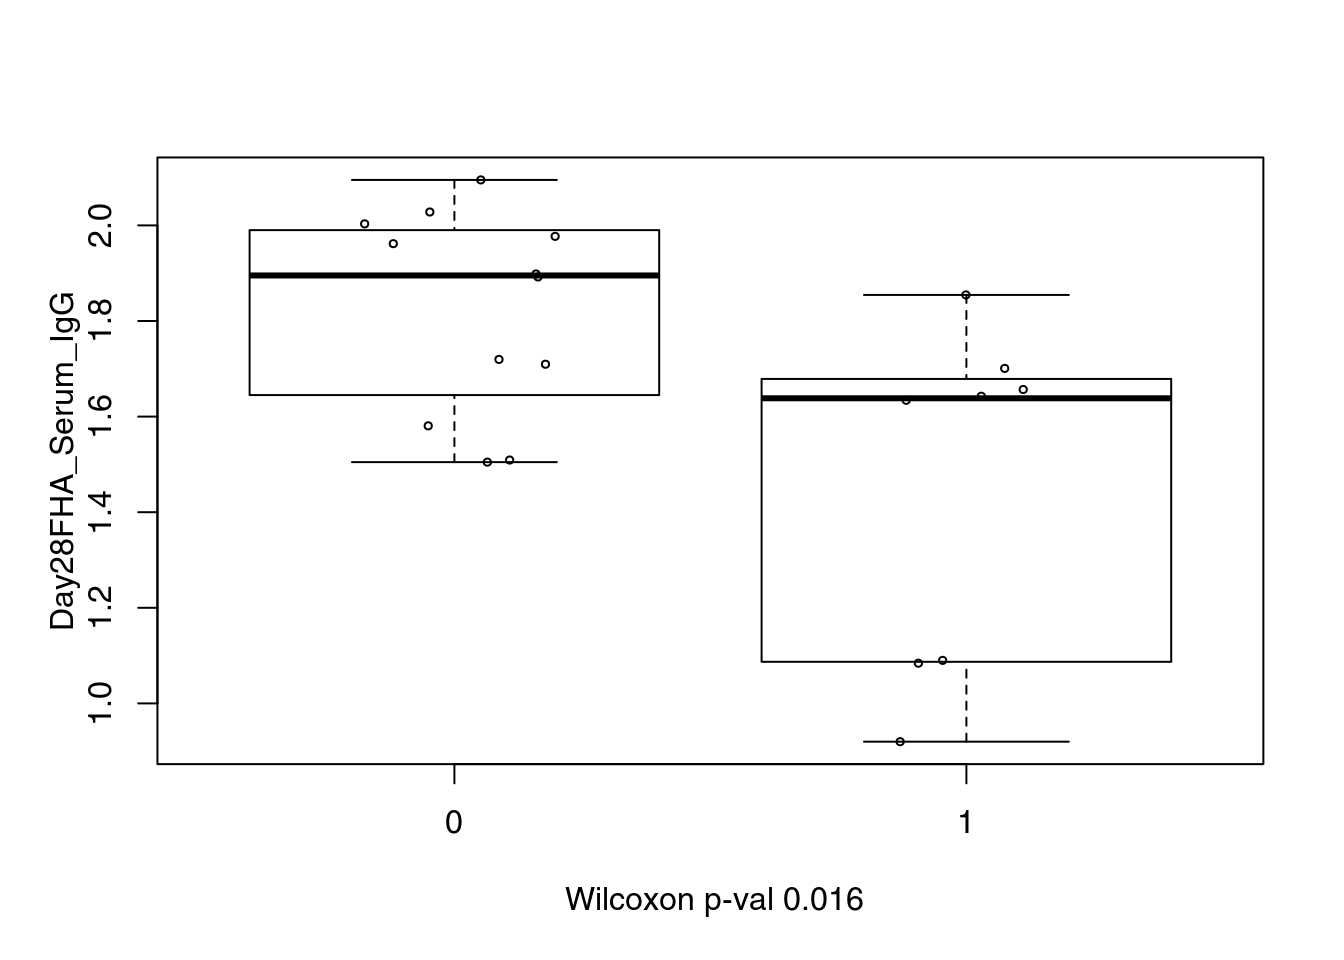
\includegraphics{posthoc_analyses_files/figure-latex/spot check p vals-1.pdf}

\begin{verbatim}
## 
##  Welch Two Sample t-test
## 
## data:  Day28FHA_Serum_IgG by EventIndC9_11_14
## t = 2.6909, df = 10.275, p-value = 0.02217
## alternative hypothesis: true difference in means is not equal to 0
## 95 percent confidence interval:
##  0.06568587 0.68515210
## sample estimates:
## mean in group 0 mean in group 1 
##        1.823251        1.447832
\end{verbatim}

\begin{verbatim}
## [[1]]
##                    1                                 
## (Intercept)        "2.71 (CI=-0.63, 6.05, p=0.112)"  
## Day28WCE_Serum_IgA "-2.03 (CI=-3.90,-0.15, p=0.034)*"
## 
## [[2]]
##                    1                               
## (Intercept)        "2.71 (CI=-2.06,7.47, p=0.266)" 
## Day28WCE_Serum_IgA "-2.03 (CI=-4.64,0.59, p=0.128)"
## 
## [[3]]
##                    1                               
## (Intercept)        "2.71 (CI=-1.00,6.41, p=0.153)" 
## Day28WCE_Serum_IgA "-2.03 (CI=-4.12,0.07, p=0.058)"
\end{verbatim}

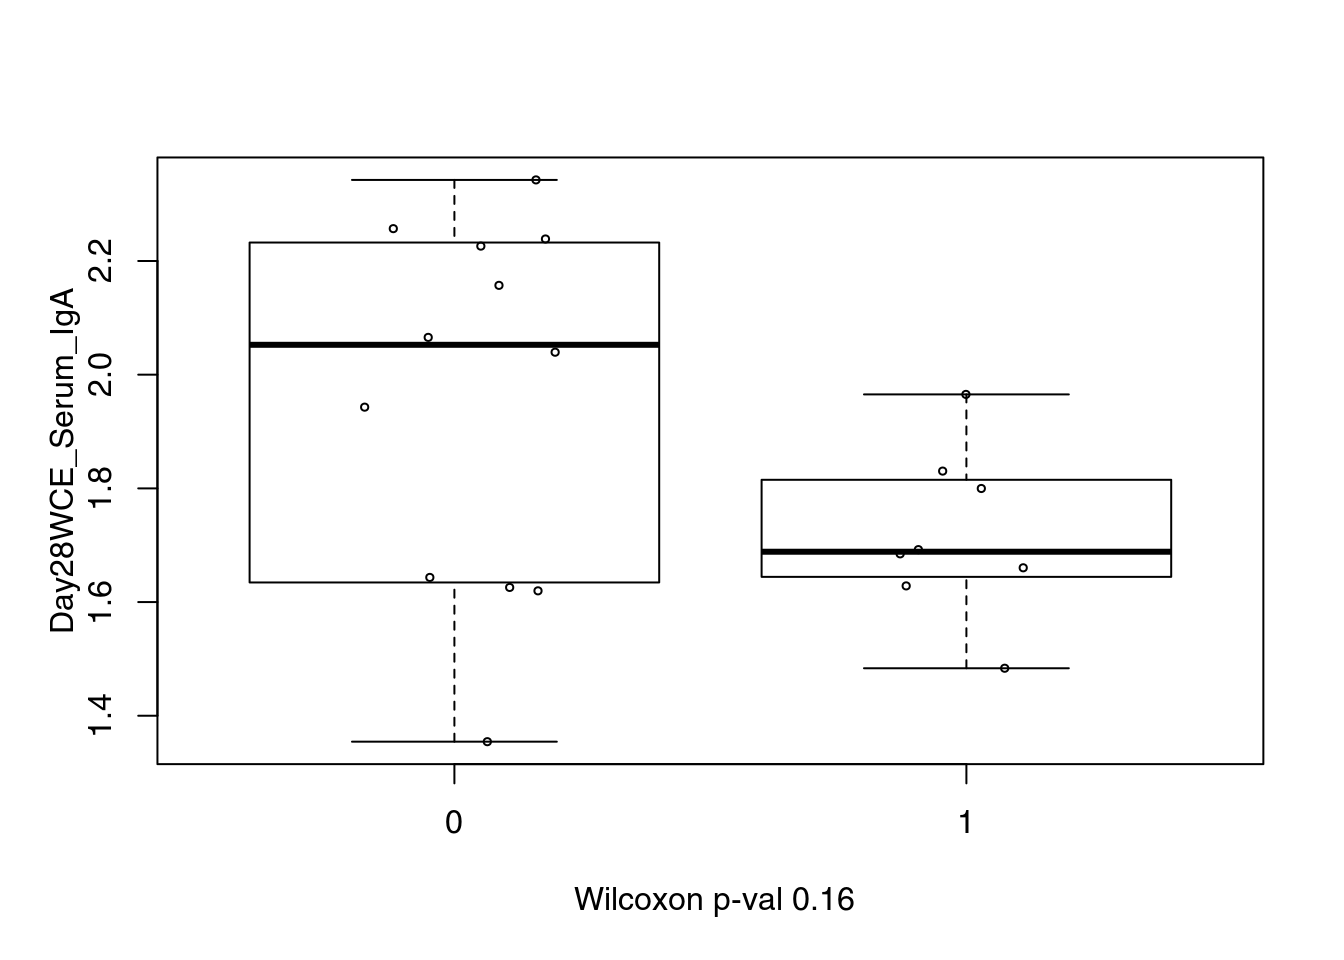
\includegraphics{posthoc_analyses_files/figure-latex/spot check p vals-2.pdf}

\begin{verbatim}
## 
##  Welch Two Sample t-test
## 
## data:  Day28WCE_Serum_IgA by EventIndC9_11_14
## t = 2.2754, df = 16.386, p-value = 0.03664
## alternative hypothesis: true difference in means is not equal to 0
## 95 percent confidence interval:
##  0.01691396 0.46565795
## sample estimates:
## mean in group 0 mean in group 1 
##        1.959380        1.718094
\end{verbatim}

\begin{verbatim}
## [[1]]
##                    1                               
## (Intercept)        "-0.65 (CI=-1.78,0.49, p=0.266)"
## Day28WCE_Nasal_IgA "-0.33 (CI=-1.70,1.04, p=0.637)"
## 
## [[2]]
##                    1                               
## (Intercept)        "-0.65 (CI=-2.06,0.77, p=0.370)"
## Day28WCE_Nasal_IgA "-0.33 (CI=-2.01,1.35, p=0.701)"
## 
## [[3]]
##                    1                               
## (Intercept)        "-0.65 (CI=-1.90,0.61, p=0.312)"
## Day28WCE_Nasal_IgA "-0.33 (CI=-1.82,1.16, p=0.665)"
\end{verbatim}

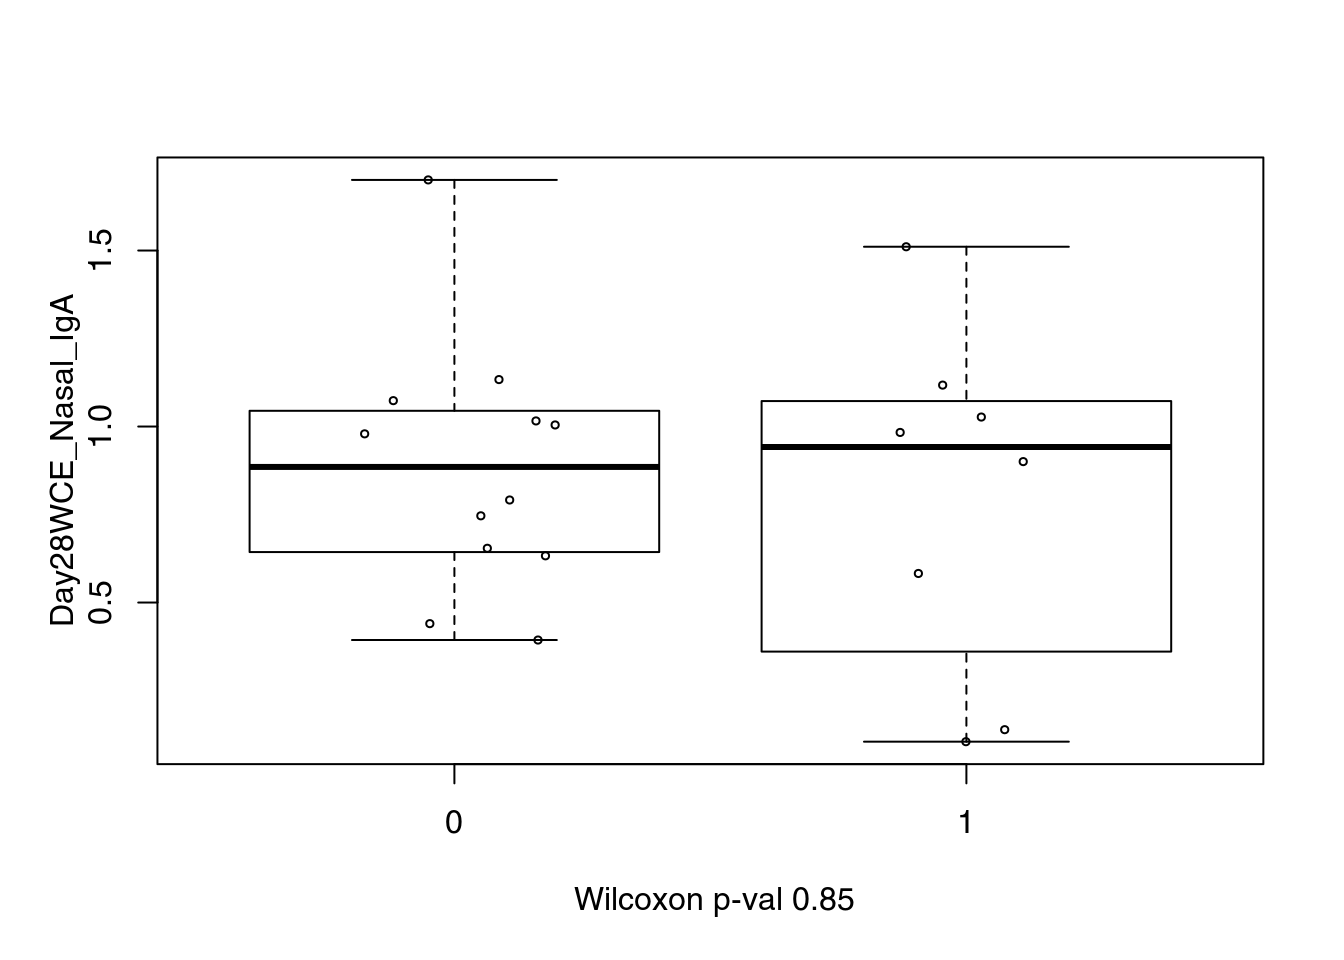
\includegraphics{posthoc_analyses_files/figure-latex/spot check p vals-3.pdf}

\begin{verbatim}
## 
##  Welch Two Sample t-test
## 
## data:  Day28WCE_Nasal_IgA by EventIndC9_11_14
## t = 0.42241, df = 11.868, p-value = 0.6803
## alternative hypothesis: true difference in means is not equal to 0
## 95 percent confidence interval:
##  -0.3531279  0.5227200
## sample estimates:
## mean in group 0 mean in group 1 
##       0.8804482       0.7956521
\end{verbatim}

\begin{verbatim}
## [[1]]
##                         1                               
## (Intercept)             "2.31 (CI=-0.71,5.33, p=0.134)" 
## Day28WCE_Norm_Nasal_IgA "-1.78 (CI=-3.62,0.06, p=0.058)"
## 
## [[2]]
##                         1                               
## (Intercept)             "2.31 (CI=-1.08,5.70, p=0.181)" 
## Day28WCE_Norm_Nasal_IgA "-1.78 (CI=-3.84,0.28, p=0.090)"
## 
## [[3]]
##                         1                               
## (Intercept)             "2.31 (CI=-1.02,5.64, p=0.175)" 
## Day28WCE_Norm_Nasal_IgA "-1.78 (CI=-3.78,0.23, p=0.082)"
\end{verbatim}

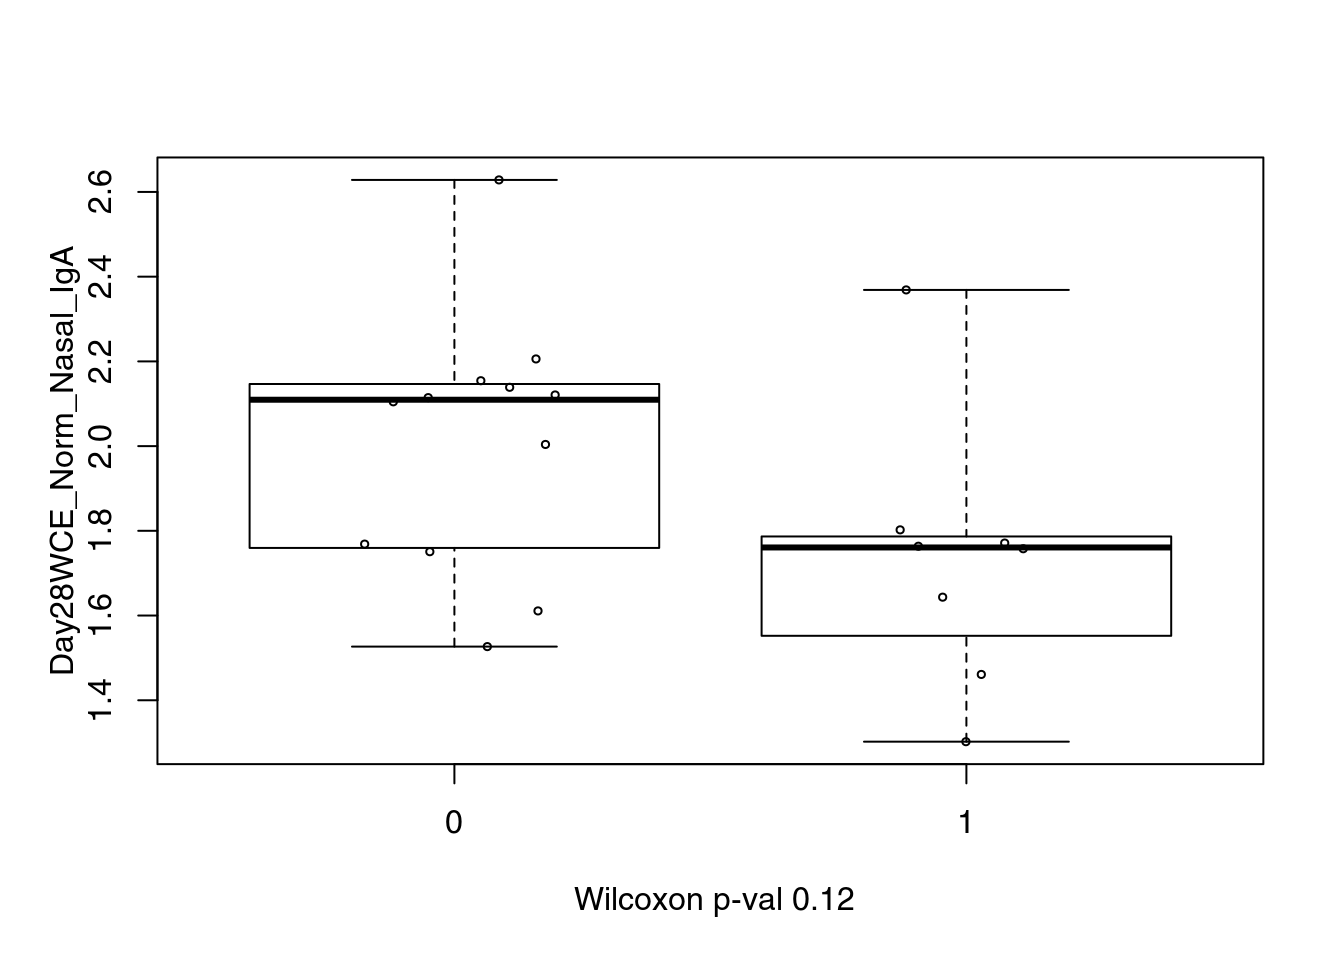
\includegraphics{posthoc_analyses_files/figure-latex/spot check p vals-4.pdf}

\begin{verbatim}
## 
##  Welch Two Sample t-test
## 
## data:  Day28WCE_Norm_Nasal_IgA by EventIndC9_11_14
## t = 1.9691, df = 14.846, p-value = 0.0679
## alternative hypothesis: true difference in means is not equal to 0
## 95 percent confidence interval:
##  -0.02310839  0.57693506
## sample estimates:
## mean in group 0 mean in group 1 
##        2.010660        1.733747
\end{verbatim}

\begin{verbatim}
## [[1]]
##                     1                                 
## (Intercept)         "-0.70 (CI=-1.34,-0.06, p=0.031)*"
## BFHA_Norm_Nasal_IgA "-0.57 (CI=-1.62, 0.49, p=0.292)" 
## 
## [[2]]
##                     1                               
## (Intercept)         "-0.70 (CI=-1.47,0.07, p=0.076)"
## BFHA_Norm_Nasal_IgA "-0.57 (CI=-1.88,0.75, p=0.400)"
## 
## [[3]]
##                     1                                
## (Intercept)         "-0.70 (CI=-1.40,0.00, p=0.049)*"
## BFHA_Norm_Nasal_IgA "-0.57 (CI=-1.73,0.60, p=0.343)"
\end{verbatim}

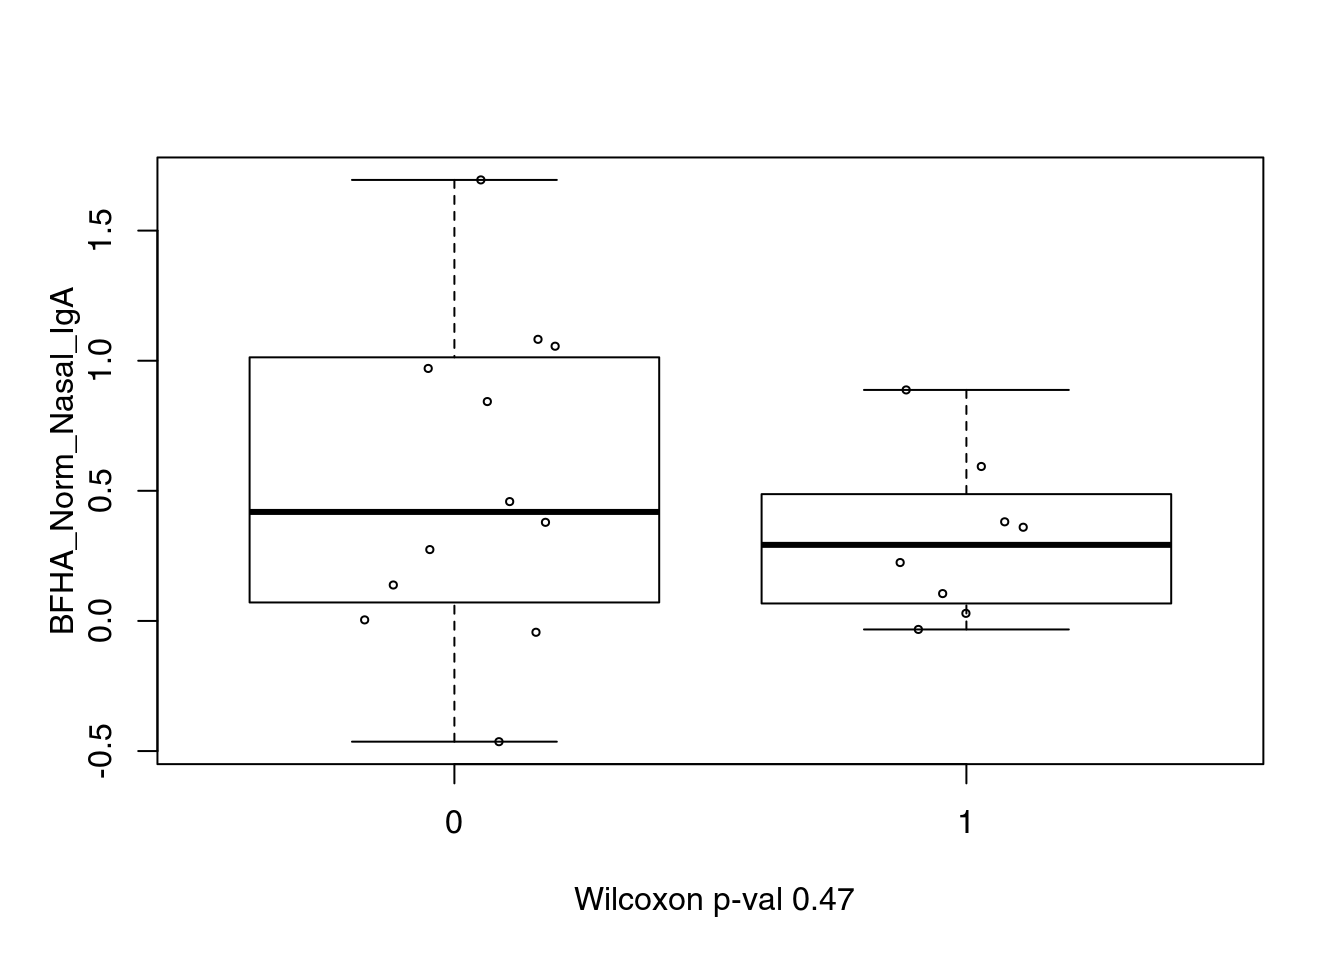
\includegraphics{posthoc_analyses_files/figure-latex/spot check p vals-5.pdf}

\begin{verbatim}
## 
##  Welch Two Sample t-test
## 
## data:  BFHA_Norm_Nasal_IgA by EventIndC9_11_14
## t = 1.0359, df = 17.123, p-value = 0.3146
## alternative hypothesis: true difference in means is not equal to 0
## 95 percent confidence interval:
##  -0.2217902  0.6501531
## sample estimates:
## mean in group 0 mean in group 1 
##       0.5326978       0.3185164
\end{verbatim}

\begin{verbatim}
## [[1]]
##                    1                                   
## (Intercept)        "2.08 (CI= 1.09, 3.06, p=<0.001)**" 
## Day28FHA_Serum_IgG "-1.92 (CI=-2.81,-1.03, p=<0.001)**"
## 
## [[2]]
##                    1                                   
## (Intercept)        "2.08 (CI= 0.90, 3.26, p=0.001)**"  
## Day28FHA_Serum_IgG "-1.92 (CI=-2.92,-0.92, p=<0.001)**"
## 
## [[3]]
##                    1                                   
## (Intercept)        "2.08 (CI= 0.84, 3.31, p=0.001)**"  
## Day28FHA_Serum_IgG "-1.92 (CI=-2.95,-0.89, p=<0.001)**"
\end{verbatim}

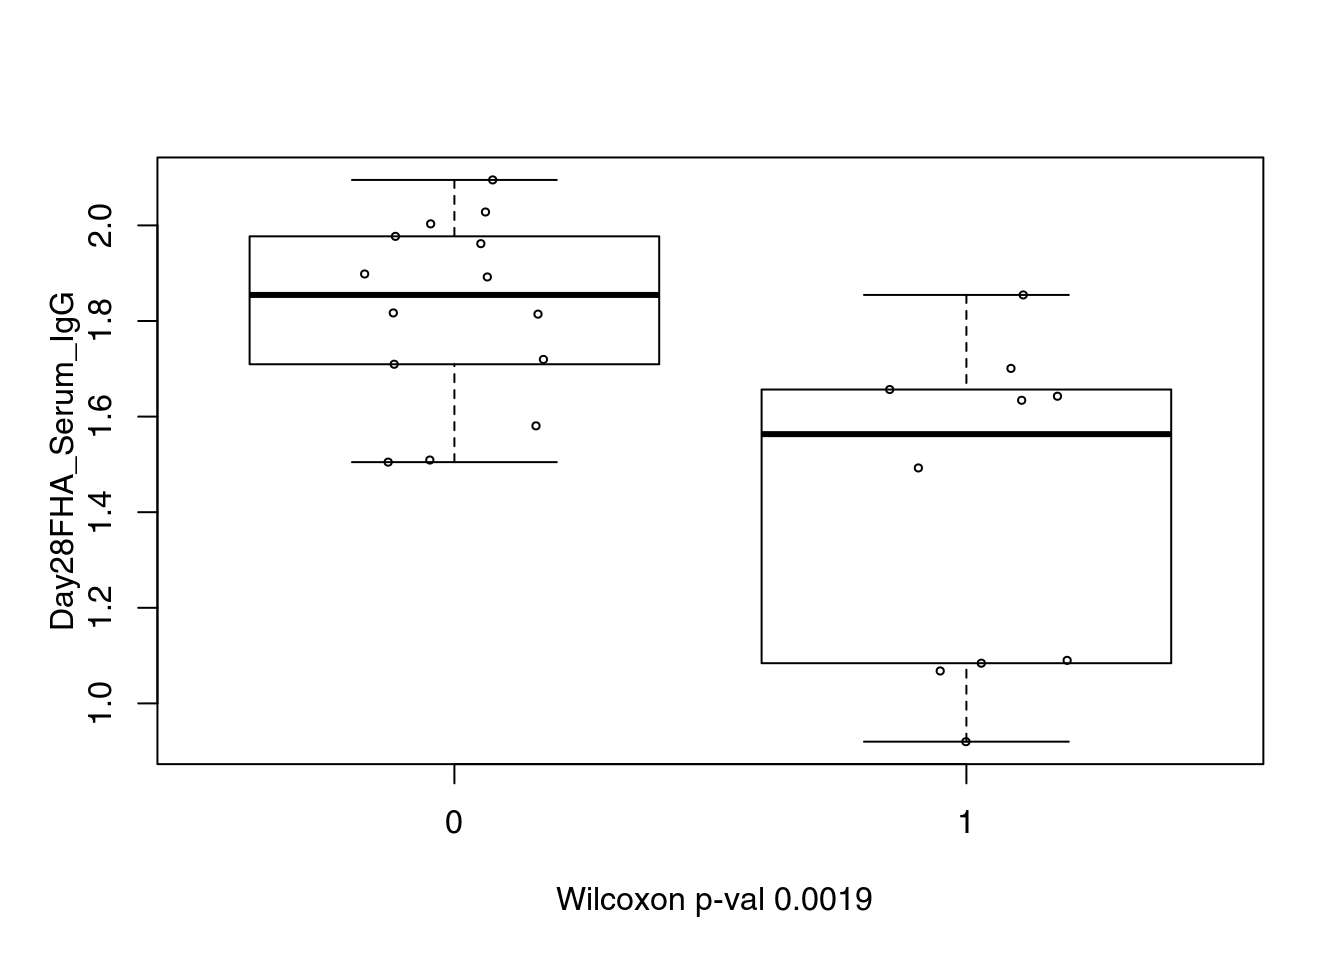
\includegraphics{posthoc_analyses_files/figure-latex/spot check p vals-6.pdf}

\begin{verbatim}
## 
##  Welch Two Sample t-test
## 
## data:  Day28FHA_Serum_IgG by EventIndC9_11_14
## t = 3.448, df = 13.218, p-value = 0.004229
## alternative hypothesis: true difference in means is not equal to 0
## 95 percent confidence interval:
##  0.1527383 0.6629601
## sample estimates:
## mean in group 0 mean in group 1 
##        1.822158        1.414308
\end{verbatim}

\begin{verbatim}
## [[1]]
##                    1                               
## (Intercept)        "-0.04 (CI=-2.46,2.37, p=0.971)"
## Day28WCE_Serum_IgA "-0.45 (CI=-1.75,0.85, p=0.495)"
## 
## [[2]]
##                    1                               
## (Intercept)        "-0.04 (CI=-3.66,3.57, p=0.981)"
## Day28WCE_Serum_IgA "-0.45 (CI=-2.36,1.45, p=0.641)"
## 
## [[3]]
##                    1                               
## (Intercept)        "-0.04 (CI=-2.64,2.55, p=0.973)"
## Day28WCE_Serum_IgA "-0.45 (CI=-1.85,0.95, p=0.526)"
\end{verbatim}

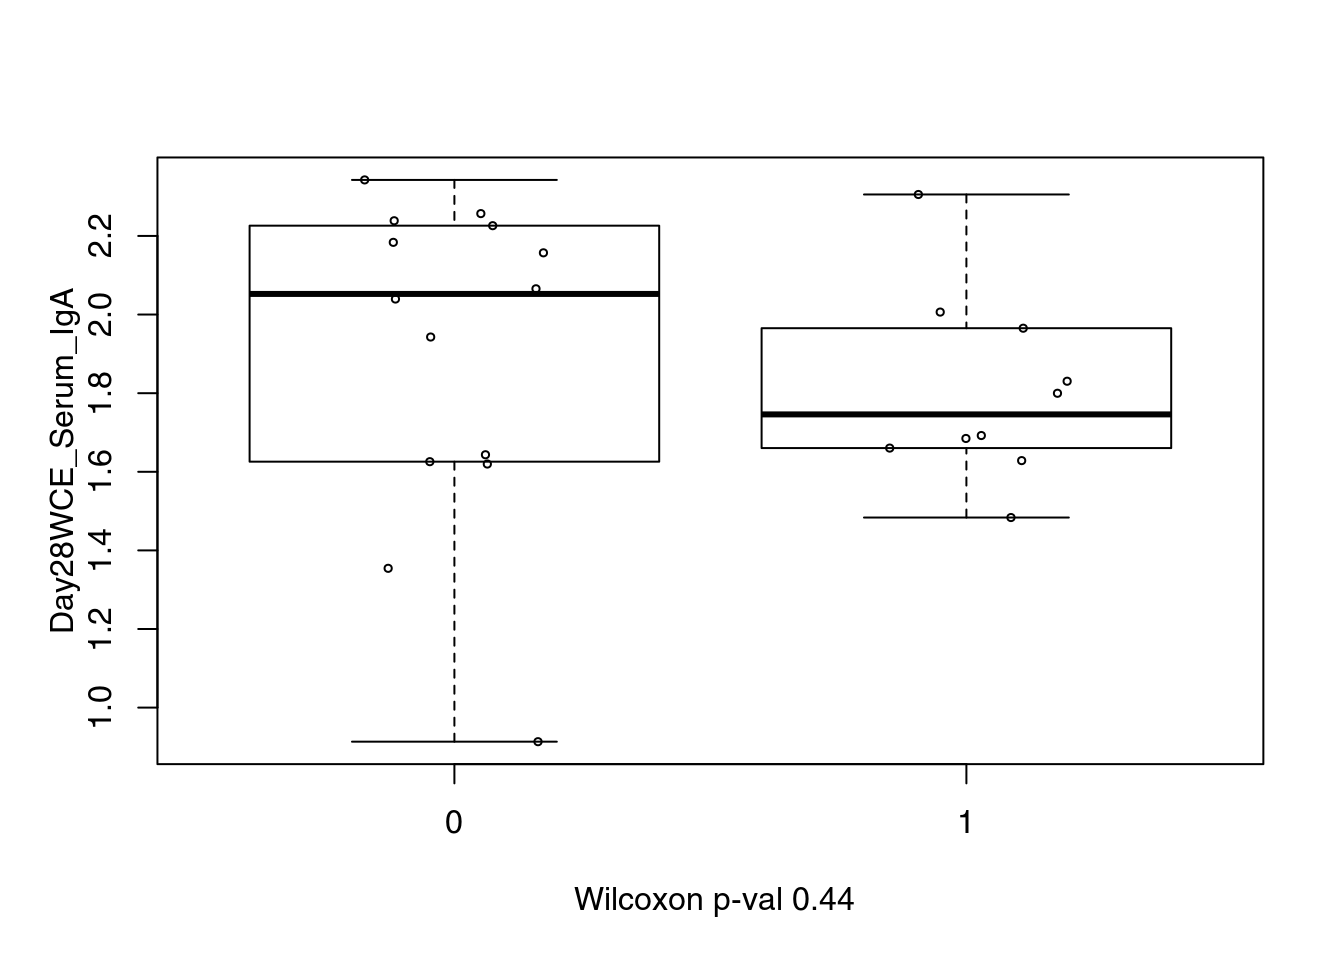
\includegraphics{posthoc_analyses_files/figure-latex/spot check p vals-7.pdf}

\begin{verbatim}
## 
##  Welch Two Sample t-test
## 
## data:  Day28WCE_Serum_IgA by EventIndC9_11_14
## t = 0.712, df = 21.173, p-value = 0.4842
## alternative hypothesis: true difference in means is not equal to 0
## 95 percent confidence interval:
##  -0.1823853  0.3724343
## sample estimates:
## mean in group 0 mean in group 1 
##        1.900685        1.805660
\end{verbatim}

\begin{verbatim}
## [[1]]
##                     1                                  
## (Intercept)         "-0.65 (CI=-1.09,-0.21, p=0.004)**"
## BFHA_Norm_Nasal_IgA "-0.78 (CI=-1.43,-0.13, p=0.019)*" 
## 
## [[2]]
##                     1                                  
## (Intercept)         "-0.65 (CI=-1.13,-0.17, p=0.008)**"
## BFHA_Norm_Nasal_IgA "-0.78 (CI=-1.50,-0.05, p=0.037)*" 
## 
## [[3]]
##                     1                                  
## (Intercept)         "-0.65 (CI=-1.13,-0.17, p=0.008)**"
## BFHA_Norm_Nasal_IgA "-0.78 (CI=-1.51,-0.04, p=0.039)*"
\end{verbatim}

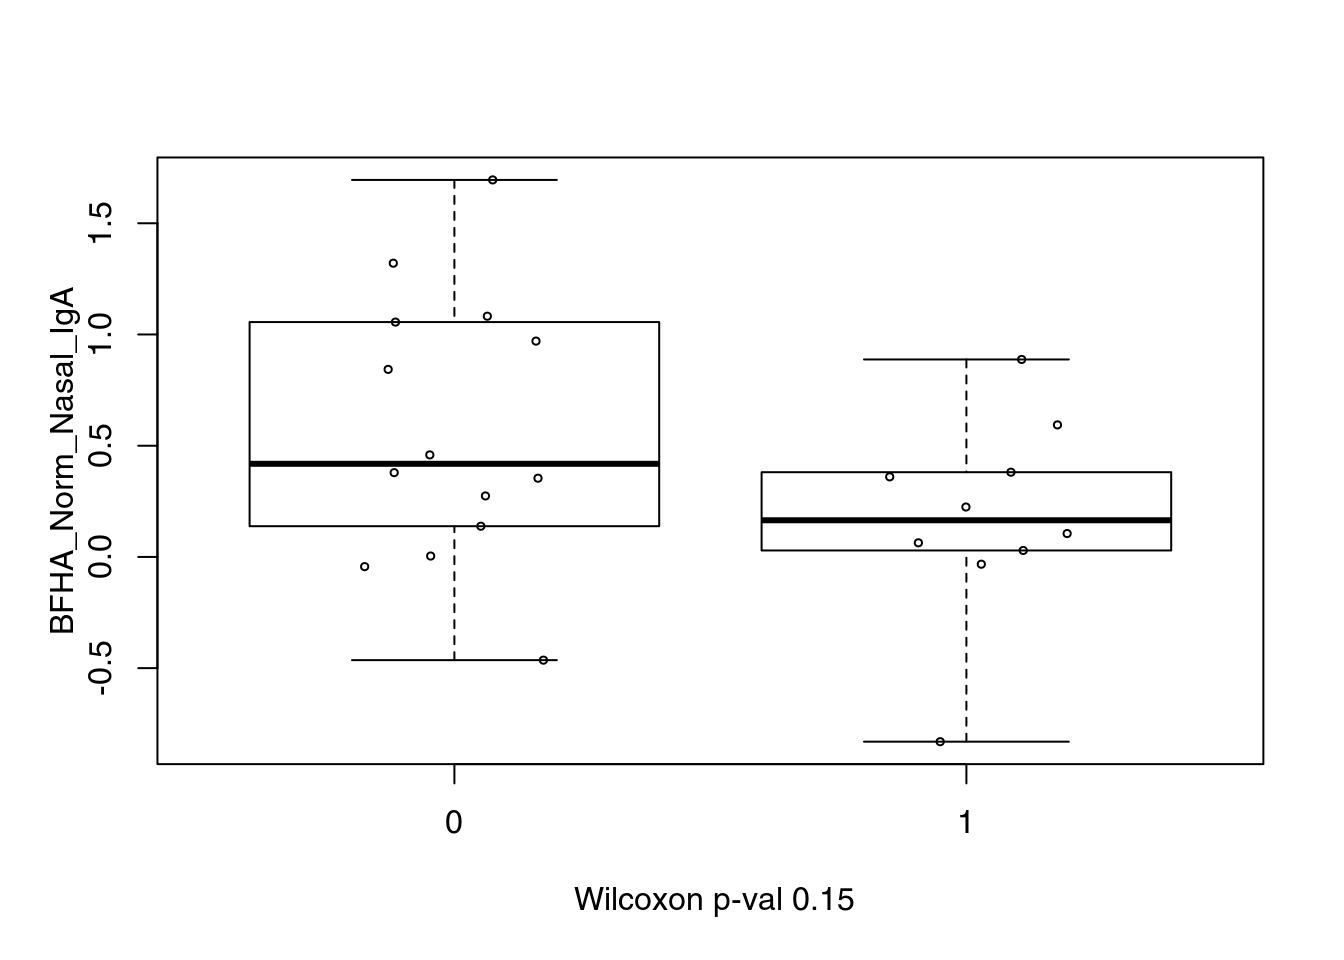
\includegraphics{posthoc_analyses_files/figure-latex/spot check p vals-8.pdf}

\begin{verbatim}
## 
##  Welch Two Sample t-test
## 
## data:  BFHA_Norm_Nasal_IgA by EventIndC9_11_14
## t = 1.8477, df = 21.889, p-value = 0.0782
## alternative hypothesis: true difference in means is not equal to 0
## 95 percent confidence interval:
##  -0.04885459  0.84504972
## sample estimates:
## mean in group 0 mean in group 1 
##       0.5761989       0.1781013
\end{verbatim}

\begin{verbatim}
## [[1]]
##                         1                                 
## (Intercept)             "-0.09 (CI=-0.24, 0.07, p=0.264)" 
## Day28FHA_Norm_Nasal_IgA "-0.63 (CI=-1.20,-0.06, p=0.029)*"
## 
## [[2]]
##                         1                               
## (Intercept)             "-0.09 (CI=-0.27,0.09, p=0.341)"
## Day28FHA_Norm_Nasal_IgA "-0.63 (CI=-1.30,0.03, p=0.062)"
## 
## [[3]]
##                         1                               
## (Intercept)             "-0.09 (CI=-0.37,0.19, p=0.540)"
## Day28FHA_Norm_Nasal_IgA "-0.63 (CI=-1.35,0.08, p=0.082)"
\end{verbatim}

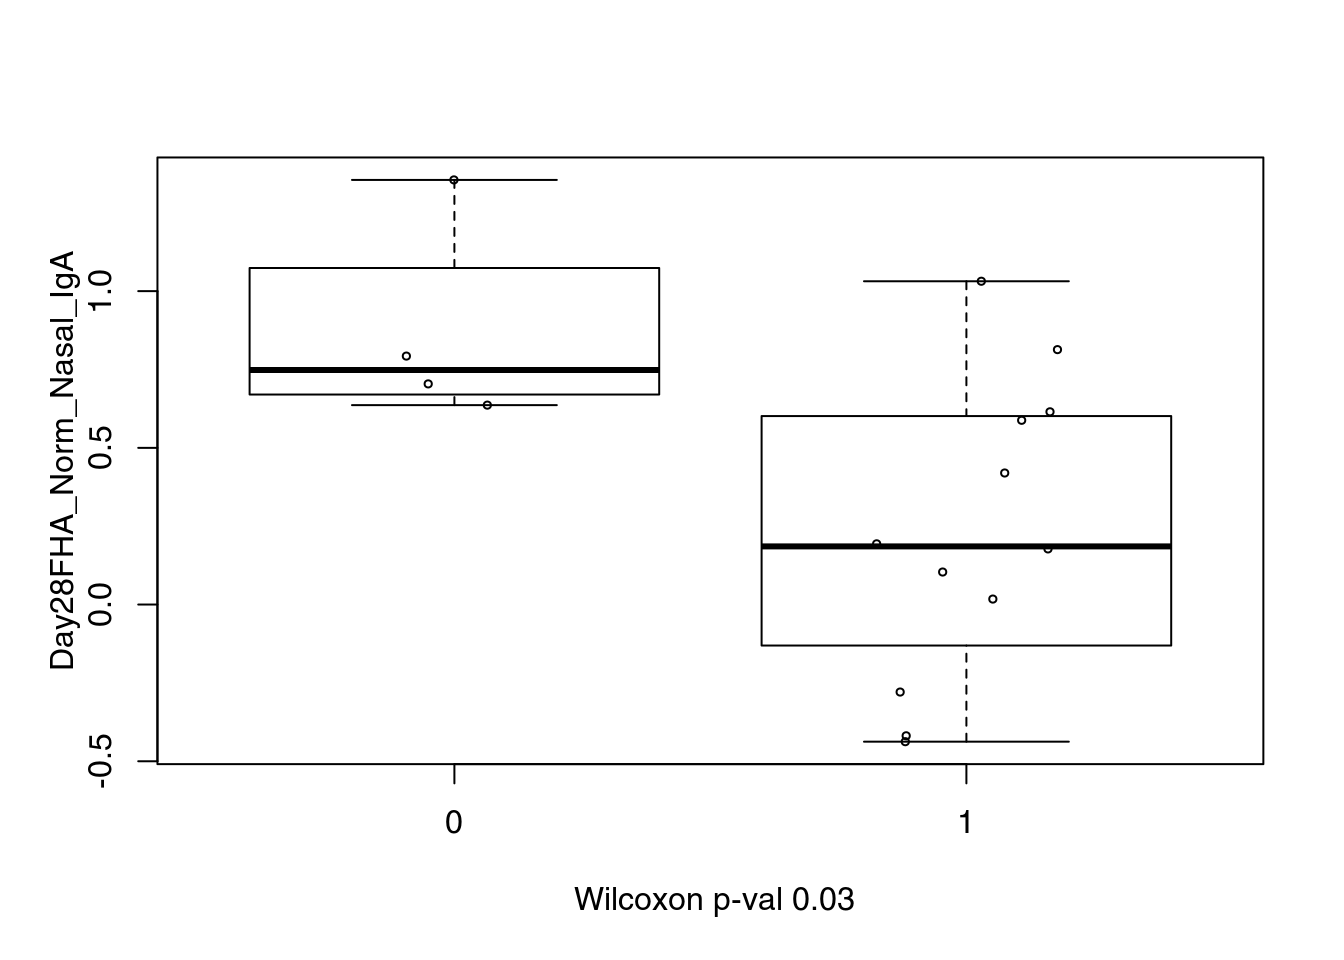
\includegraphics{posthoc_analyses_files/figure-latex/spot check p vals-9.pdf}

\begin{verbatim}
## 
##  Welch Two Sample t-test
## 
## data:  Day28FHA_Norm_Nasal_IgA by EventIndC9_11_14
## t = 2.9758, df = 7.6423, p-value = 0.01865
## alternative hypothesis: true difference in means is not equal to 0
## 95 percent confidence interval:
##  0.1392521 1.1340412
## sample estimates:
## mean in group 0 mean in group 1 
##       0.8719862       0.2353395
\end{verbatim}

\begin{verbatim}
## [[1]]
##                     1                                 
## (Intercept)         "-0.13 (CI=-0.32, 0.06, p=0.196)" 
## BFHA_Norm_Nasal_IgA "-0.65 (CI=-1.16,-0.14, p=0.012)*"
## 
## [[2]]
##                     1                                 
## (Intercept)         "-0.13 (CI=-0.35, 0.10, p=0.278)" 
## BFHA_Norm_Nasal_IgA "-0.65 (CI=-1.26,-0.04, p=0.036)*"
## 
## [[3]]
##                     1                                
## (Intercept)         "-0.13 (CI=-0.42,0.17, p=0.400)" 
## BFHA_Norm_Nasal_IgA "-0.65 (CI=-1.30,0.00, p=0.048)*"
\end{verbatim}

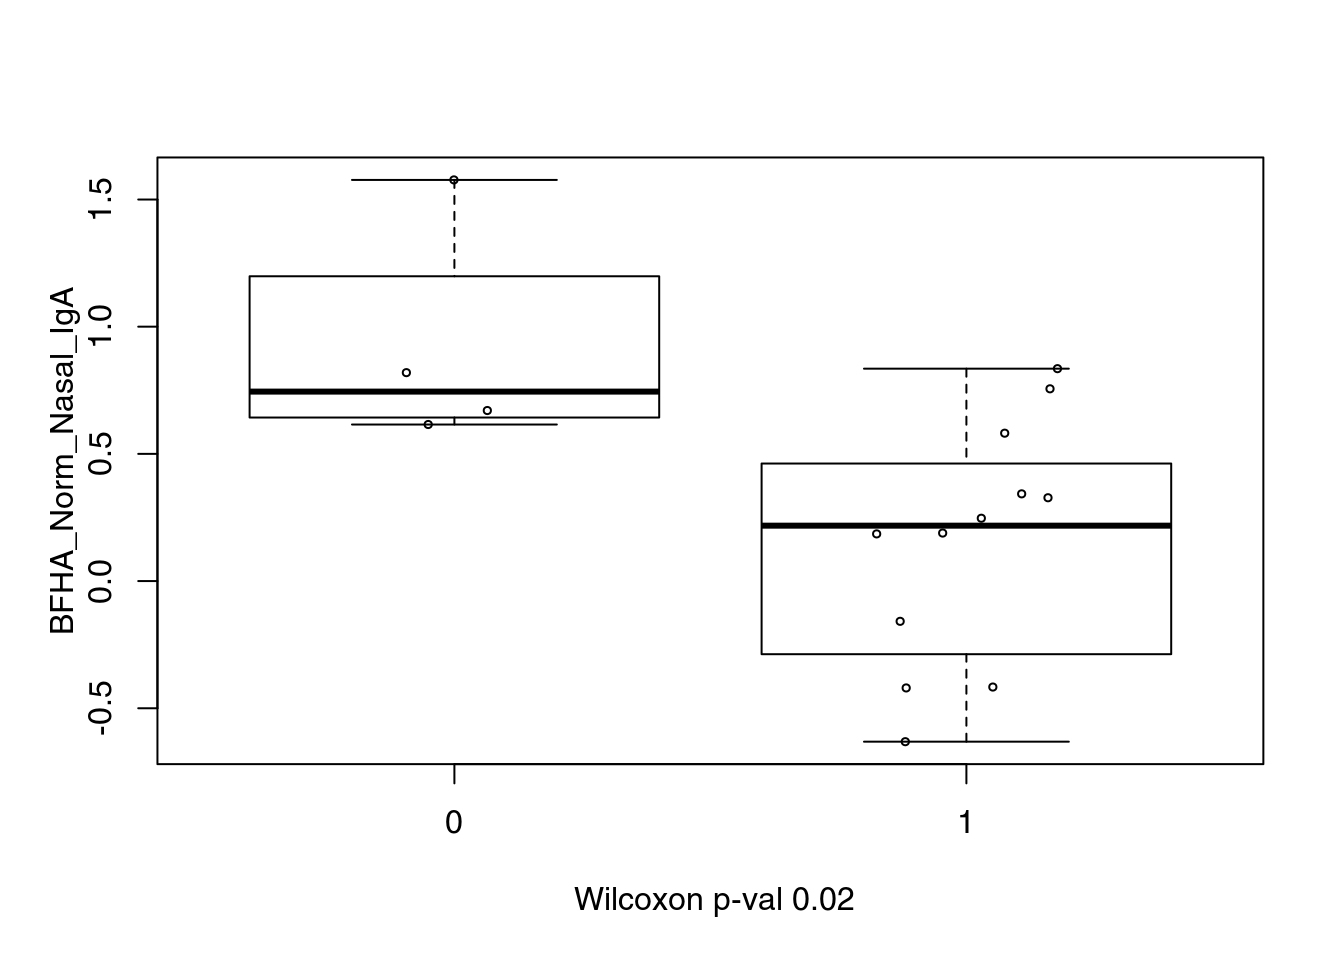
\includegraphics{posthoc_analyses_files/figure-latex/spot check p vals-10.pdf}

\begin{verbatim}
## 
##  Welch Two Sample t-test
## 
## data:  BFHA_Norm_Nasal_IgA by EventIndC9_11_14
## t = 2.936, df = 5.455, p-value = 0.02919
## alternative hypothesis: true difference in means is not equal to 0
## 95 percent confidence interval:
##  0.1120295 1.4229709
## sample estimates:
## mean in group 0 mean in group 1 
##       0.9205663       0.1530661
\end{verbatim}

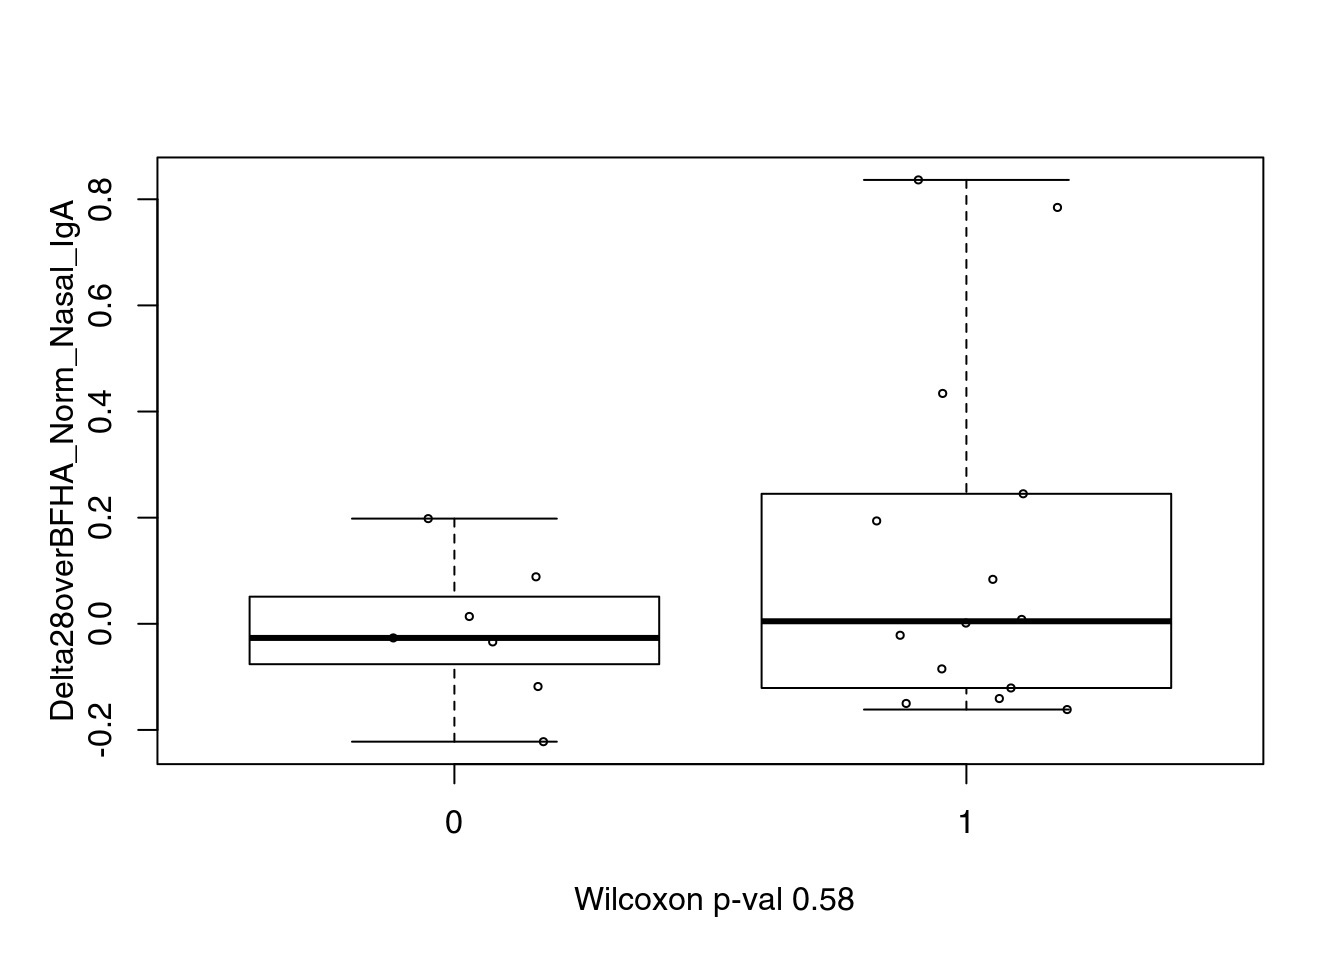
\includegraphics{posthoc_analyses_files/figure-latex/exploratory spot check wilcox robust binomial-1.pdf}

\begin{verbatim}
##                                1                                  
## (Intercept)                    "-0.47 (CI=-0.82,-0.11, p=0.010)**"
## Delta28overBFHA_Norm_Nasal_IgA "0.56 (CI=-0.02, 1.14, p=0.056)"
\end{verbatim}

\begin{verbatim}
##                                1                               
## (Intercept)                    "-0.47 (CI=-1.04,0.10, p=0.108)"
## Delta28overBFHA_Norm_Nasal_IgA "0.56 (CI=-1.10,2.23, p=0.506)"
\end{verbatim}

\begin{verbatim}
##                                1                              
## (Intercept)                    "0.57 (CI=-0.38,1.52, p=0.240)"
## Delta28overBFHA_Norm_Nasal_IgA "2.61 (CI=-0.64,5.86, p=0.116)"
\end{verbatim}

\begin{verbatim}
##                                1                              
## (Intercept)                    "0.57 (CI=-0.37,1.51, p=0.235)"
## Delta28overBFHA_Norm_Nasal_IgA "2.61 (CI=-2.15,7.37, p=0.283)"
\end{verbatim}

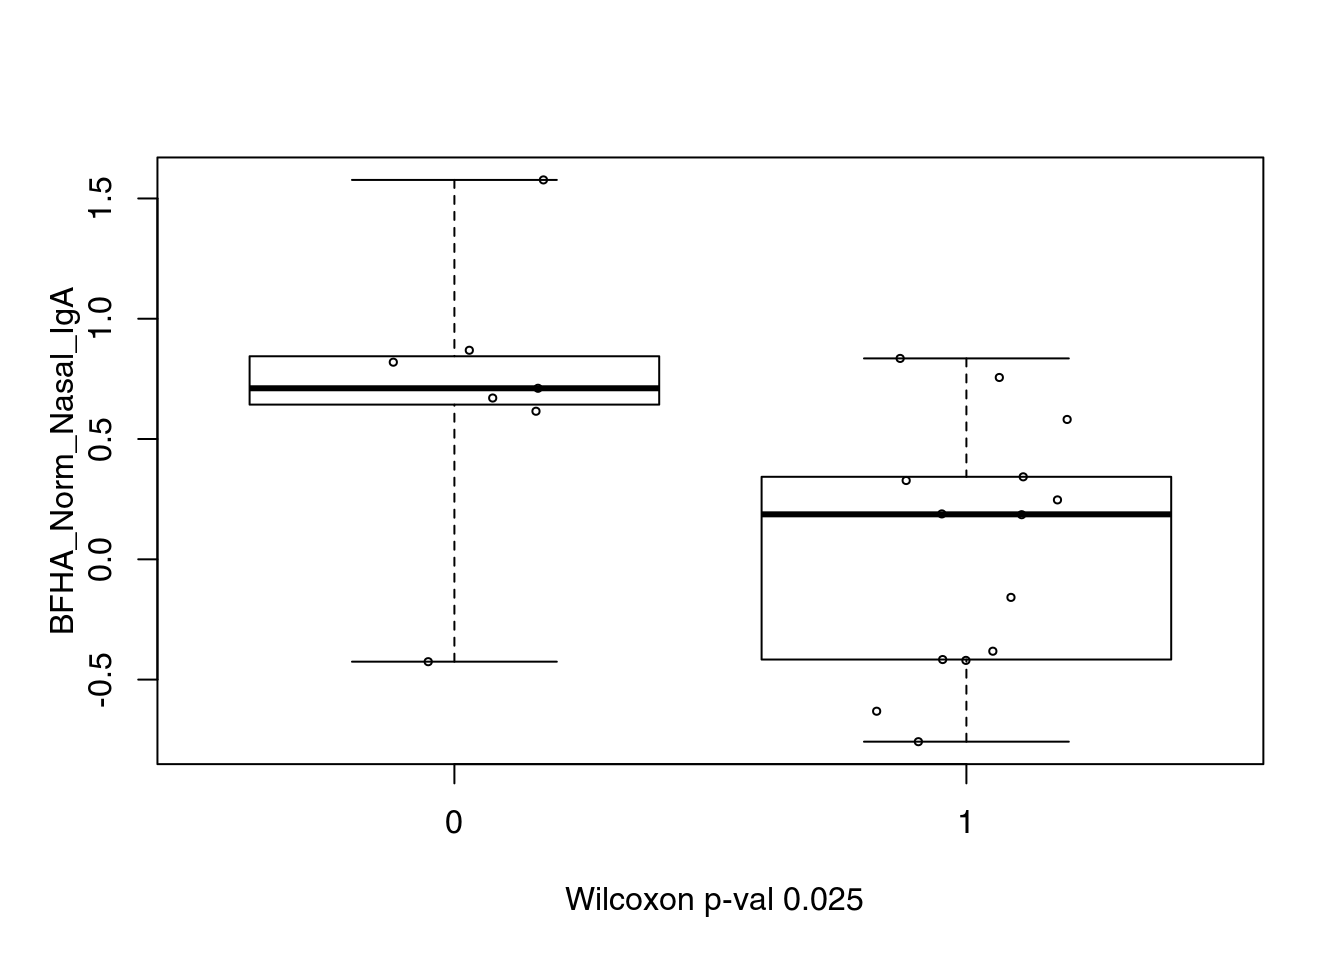
\includegraphics{posthoc_analyses_files/figure-latex/exploratory spot check wilcox robust binomial-2.pdf}

\begin{verbatim}
##                     1              
## (Intercept)         "-0.31 (0.13)*"
## BFHA_Norm_Nasal_IgA "-0.62 (0.25)*"
\end{verbatim}

\begin{verbatim}
##                     1             
## (Intercept)         "-0.31 (0.27)"
## BFHA_Norm_Nasal_IgA "-0.62 (0.46)"
\end{verbatim}

\begin{verbatim}
## $NO
##            [,1]       [,2]
## [1,] 0.01821786 0.01022190
## [2,] 0.01022190 0.07936095
## 
## $MBN
##            [,1]       [,2]
## [1,] 0.02181814 0.00797982
## [2,] 0.00797982 0.08787044
## 
## $MD
##            [,1]       [,2]
## [1,] 0.02165160 0.01158637
## [2,] 0.01158637 0.11845727
## 
## $KC
##            [,1]       [,2]
## [1,] 0.01821786 0.01022190
## [2,] 0.01022190 0.07936095
## 
## $mFG
##            [,1]       [,2]
## [1,] 0.01985218 0.01088325
## [2,] 0.01088325 0.09629685
\end{verbatim}

\begin{verbatim}
##                     1              
## (Intercept)         "-0.31 (0.13)*"
## BFHA_Norm_Nasal_IgA "-0.62 (0.25)*"
\end{verbatim}

\begin{verbatim}
##                     1                               
## (Intercept)         "1.66 (CI=-0.35,3.68, p=0.106)" 
## BFHA_Norm_Nasal_IgA "-2.50 (CI=-5.58,0.58, p=0.111)"
\end{verbatim}

\begin{verbatim}
##                     1                               
## (Intercept)         "1.66 (CI= 0.05,3.28, p=0.044)*"
## BFHA_Norm_Nasal_IgA "-2.50 (CI=-5.02,0.01, p=0.051)"
\end{verbatim}

\begin{verbatim}
## Beginning Cgee S-function, @(#) geeformula.q 4.13 98/01/27
\end{verbatim}

\begin{verbatim}
## running glm to get initial regression estimate
\end{verbatim}

\begin{verbatim}
##         (Intercept) BFHA_Norm_Nasal_IgA 
##          -0.3094165          -0.6176155
\end{verbatim}

\begin{verbatim}
## [1] 0.1580692 0.2732594
\end{verbatim}

\begin{verbatim}
## [1] 0.1318070 0.2510843
\end{verbatim}

\begin{verbatim}
## [1] 0.1318070 0.2510843
\end{verbatim}

\begin{verbatim}
## [1] 0.1318070 0.2510843
\end{verbatim}

\begin{verbatim}
## [1] 0.1348993 0.2599329
\end{verbatim}

\begin{verbatim}
## [1] 0.1348993 0.2599329
\end{verbatim}

\begin{verbatim}
## Beginning Cgee S-function, @(#) geeformula.q 4.13 98/01/27
## running glm to get initial regression estimate
\end{verbatim}

\begin{verbatim}
##                    (Intercept) Delta28overBFHA_Norm_Nasal_IgA 
##                     -0.4676743                      0.5645808
\end{verbatim}

\begin{verbatim}
## [1] 0.1810117 0.2957376
\end{verbatim}

\begin{verbatim}
## [1] 0.1810117 0.2957376
\end{verbatim}

\begin{verbatim}
## [1] 0.1810117 0.2957376
\end{verbatim}

\begin{verbatim}
## [1] 0.1859998 0.3021185
\end{verbatim}

\begin{verbatim}
## [1] 0.1859998 0.3021185
\end{verbatim}

\begin{verbatim}
## Beginning Cgee S-function, @(#) geeformula.q 4.13 98/01/27
## running glm to get initial regression estimate
\end{verbatim}

\begin{verbatim}
##                    (Intercept) Delta28overBFHA_Norm_Nasal_IgA 
##                      0.6301523                      0.4243456
\end{verbatim}

\begin{verbatim}
## [1] 0.1108851 0.2052113
\end{verbatim}

\begin{verbatim}
## [1] 0.1108851 0.2052113
\end{verbatim}

\begin{verbatim}
## [1] 0.1108851 0.2052113
\end{verbatim}

\begin{verbatim}
## [1] 0.1139483 0.2097095
\end{verbatim}

\begin{verbatim}
## [1] 0.1139483 0.2097095
\end{verbatim}

\begin{verbatim}
##          [,1]      [,2]
## NO  0.1108851 0.2052113
## MBN 0.1159142 0.2352272
## MD  0.1188056 0.2241034
## KC  0.1108851 0.2052113
## mFG 0.1147668 0.2143640
\end{verbatim}

\begin{tabular}{>{}l|>{}c|>{}c|>{}c|c}
\hline
\multicolumn{1}{c|}{PPAI prim} & \multicolumn{1}{c|}{Nasal\_IgA} & \multicolumn{1}{c|}{Norm\_Nasal\_IgA} & \multicolumn{1}{c|}{Serum\_IgA} & \multicolumn{1}{c}{Serum\_IgG} \\
\cline{1-1} \cline{2-2} \cline{3-3} \cline{4-4} \cline{5-5}
B & 0.95 (0.903) & 0.79 (0.546) & 0.91 (0.822) & 1.09 (0.880)\\
\hline
Day28 & 0.86 (0.722) & 0.44 (0.055) & 0.49 (0.068) & 0.65 (0.338)\\
\hline
Delta28overB & 0.94 (0.853) & 0.82 (0.484) & 0.58 (0.242) & 0.65 (0.388)\\
\hline
\end{tabular}

\begin{tabular}{>{}l|>{}c|>{}c|>{}c|c}
\hline
\multicolumn{1}{c|}{PP prim} & \multicolumn{1}{c|}{Nasal\_IgA} & \multicolumn{1}{c|}{Norm\_Nasal\_IgA} & \multicolumn{1}{c|}{Serum\_IgA} & \multicolumn{1}{c}{Serum\_IgG} \\
\cline{1-1} \cline{2-2} \cline{3-3} \cline{4-4} \cline{5-5}
B & 0.84 (0.625) & 0.68 (0.150) & 1.00 (0.997) & 0.90 (0.845)\\
\hline
Day28 & 0.81 (0.544) & 0.66 (0.246) & 0.91 (0.770) & 0.88 (0.758)\\
\hline
Delta28overB & 0.97 (0.914) & 1.02 (0.929) & 0.89 (0.748) & 0.95 (0.888)\\
\hline
\end{tabular}

\begin{tabular}{>{}l|>{}c|>{}c|>{}c|c}
\hline
\multicolumn{1}{c|}{PP alt} & \multicolumn{1}{c|}{Nasal\_IgA} & \multicolumn{1}{c|}{Norm\_Nasal\_IgA} & \multicolumn{1}{c|}{Serum\_IgA} & \multicolumn{1}{c}{Serum\_IgG} \\
\cline{1-1} \cline{2-2} \cline{3-3} \cline{4-4} \cline{5-5}
B & 0.70 (0.419) & 0.66 (0.244) & 0.90 (0.794) & 0.92 (0.907)\\
\hline
Day28 & 0.45 (0.079) & 0.40 (0.079) & 0.64 (0.275) & 1.21 (0.697)\\
\hline
Delta28overB & 0.78 (0.464) & 0.87 (0.634) & 0.68 (0.396) & 1.22 (0.652)\\
\hline
\end{tabular}

\begin{tabular}{>{}l|>{}c|>{}c|>{}c|c}
\hline
\multicolumn{1}{c|}{PPAI alt} & \multicolumn{1}{c|}{Nasal\_IgA} & \multicolumn{1}{c|}{Norm\_Nasal\_IgA} & \multicolumn{1}{c|}{Serum\_IgA} & \multicolumn{1}{c}{Serum\_IgG} \\
\cline{1-1} \cline{2-2} \cline{3-3} \cline{4-4} \cline{5-5}
B & 0.84 (0.724) & 0.92 (0.859) & 0.94 (0.879) & 1.04 (0.953)\\
\hline
Day28 & 0.52 (0.185) & 0.36 (0.110) & 0.39 (0.082) & 1.19 (0.745)\\
\hline
Delta28overB & 0.77 (0.476) & 0.71 (0.318) & 0.44 (0.100) & 1.13 (0.802)\\
\hline
\end{tabular}

\begin{tabular}{>{}l|>{}c|>{}c|>{}c|c}
\hline
\multicolumn{1}{c|}{PPAI} & \multicolumn{1}{c|}{Nasal\_IgA} & \multicolumn{1}{c|}{Norm\_Nasal\_IgA} & \multicolumn{1}{c|}{Serum\_IgA} & \multicolumn{1}{c}{Serum\_IgG} \\
\cline{1-1} \cline{2-2} \cline{3-3} \cline{4-4} \cline{5-5}
B & 0.65 (0.058) & 0.67 (0.067) & 1.00 (0.998) & 0.96 (0.879)\\
\hline
Day28 & 0.87 (0.555) & 0.64 (0.073) & 1.08 (0.692) & 1.06 (0.809)\\
\hline
Delta28overB & 1.35 (0.282) & 1.46 (0.353) & 2.73 (0.178) & 1.20 (0.667)\\
\hline
\end{tabular}

\begin{tabular}{>{}l|>{}c|>{}c|>{}c|c}
\hline
\multicolumn{1}{c|}{PP} & \multicolumn{1}{c|}{Nasal\_IgA} & \multicolumn{1}{c|}{Norm\_Nasal\_IgA} & \multicolumn{1}{c|}{Serum\_IgA} & \multicolumn{1}{c}{Serum\_IgG} \\
\cline{1-1} \cline{2-2} \cline{3-3} \cline{4-4} \cline{5-5}
B & 0.62 (0.035) & 0.63 (0.034) & 0.95 (0.805) & 0.75 (0.191)\\
\hline
Day28 & 0.87 (0.555) & 0.60 (0.037) & 1.03 (0.872) & 0.85 (0.492)\\
\hline
Delta28overB & 1.50 (0.225) & 1.56 (0.184) & 3.92 (0.051) & 1.27 (0.650)\\
\hline
\end{tabular}

\begin{tabular}{>{}l|>{}c|>{}c|>{}c|c}
\hline
\multicolumn{1}{c|}{PPAI prim} & \multicolumn{1}{c|}{Nasal\_IgA} & \multicolumn{1}{c|}{Norm\_Nasal\_IgA} & \multicolumn{1}{c|}{Serum\_IgA} & \multicolumn{1}{c}{Serum\_IgG} \\
\cline{1-1} \cline{2-2} \cline{3-3} \cline{4-4} \cline{5-5}
TrtBPZE1 & 0.67 (0.399) & 1.47 (0.450) & 0.62 (0.227) & 0.57 (0.125)\\
\hline
Day28Nasal\_IgA\_PC1 & 0.87 (0.478) & 0.56 (0.006) & 0.82 (0.335) & 0.90 (0.607)\\
\hline
\end{tabular}

\begin{tabular}{>{}l|>{}c|>{}c|>{}c|c}
\hline
\multicolumn{1}{c|}{PPAI alt} & \multicolumn{1}{c|}{Nasal\_IgA} & \multicolumn{1}{c|}{Norm\_Nasal\_IgA} & \multicolumn{1}{c|}{Serum\_IgA} & \multicolumn{1}{c}{Serum\_IgG} \\
\cline{1-1} \cline{2-2} \cline{3-3} \cline{4-4} \cline{5-5}
TrtBPZE1 & 0.62 (0.389) & 1.15 (0.810) & 0.47 (0.104) & 0.38 (0.019)\\
\hline
Day28Nasal\_IgA\_PC1 & 0.76 (0.224) & 0.55 (0.011) & 0.81 (0.361) & 1.10 (0.680)\\
\hline
\end{tabular}

\begin{tabular}{>{}l|>{}c|>{}c|>{}c|c}
\hline
\multicolumn{1}{c|}{PP prim} & \multicolumn{1}{c|}{Nasal\_IgA} & \multicolumn{1}{c|}{Norm\_Nasal\_IgA} & \multicolumn{1}{c|}{Serum\_IgA} & \multicolumn{1}{c}{Serum\_IgG} \\
\cline{1-1} \cline{2-2} \cline{3-3} \cline{4-4} \cline{5-5}
TrtBPZE1 & 0.82 (0.655) & 1.34 (0.505) & 0.64 (0.199) & 0.68 (0.235)\\
\hline
Day28Nasal\_IgA\_PC1 & 0.85 (0.394) & 0.63 (0.027) & 0.98 (0.893) & 0.86 (0.471)\\
\hline
\end{tabular}

\begin{tabular}{>{}l|>{}c|>{}c|>{}c|c}
\hline
\multicolumn{1}{c|}{PP alt} & \multicolumn{1}{c|}{Nasal\_IgA} & \multicolumn{1}{c|}{Norm\_Nasal\_IgA} & \multicolumn{1}{c|}{Serum\_IgA} & \multicolumn{1}{c}{Serum\_IgG} \\
\cline{1-1} \cline{2-2} \cline{3-3} \cline{4-4} \cline{5-5}
TrtBPZE1 & 0.77 (0.625) & 1.28 (0.631) & 0.51 (0.109) & 0.47 (0.052)\\
\hline
Day28Nasal\_IgA\_PC1 & 0.73 (0.147) & 0.52 (0.005) & 0.89 (0.544) & 0.94 (0.779)\\
\hline
\end{tabular}

\begin{tabular}{>{}l|>{}c|>{}c|>{}c|c}
\hline
\multicolumn{1}{c|}{PPAI prim} & \multicolumn{1}{c|}{Nasal\_IgA} & \multicolumn{1}{c|}{Norm\_Nasal\_IgA} & \multicolumn{1}{c|}{Serum\_IgA} & \multicolumn{1}{c}{Serum\_IgG} \\
\cline{1-1} \cline{2-2} \cline{3-3} \cline{4-4} \cline{5-5}
TrtBPZE1 & 0.53 (0.058) & 0.59 (0.121) & 0.53 (0.062) & 0.53 (0.066)\\
\hline
BNasal\_IgA\_PC1 & 0.74 (0.110) & 0.71 (0.065) & 0.96 (0.849) & 1.00 (0.994)\\
\hline
\end{tabular}

\begin{tabular}{>{}l|c}
\hline
  & TrtBPZE1\\
\hline
PPAI prim & 0.53 (0.056)\\
\hline
PPAI alt & 0.40 (0.019)\\
\hline
PP prim & 0.62 (0.117)\\
\hline
PP alt & 0.46 (0.032)\\
\hline
\end{tabular}

\includegraphics{posthoc_analyses_files/figure-latex/pc1 scatterplot-1.pdf}

\includegraphics{posthoc_analyses_files/figure-latex/boxplot pc1-1.pdf}

\end{document}
